%Este trabalho está licenciado sob a Licença Atribuição-CompartilhaIgual 4.0 Internacional Creative Commons. Para visualizar uma cópia desta licença, visite http://creativecommons.org/licenses/by-sa/4.0/deed.pt_BR ou mande uma carta para Creative Commons, PO Box 1866, Mountain View, CA 94042, USA.

\chapter{Problema de Valor Inicial}\label{cap_pvi}
\thispagestyle{fancy}

Neste capítulo, discutimos sobre \hl{técnicas numéricas para aproximar a solução de Equações Diferenciais Ordinárias com valor inicial (condição inicial)}, i.e. problemas da forma
\begin{subequations}\hleq
  \begin{align}
    \pmb{y}'(t) &= \pmb{f}(t,\pmb{y}(t)),\quad t>t_0,\\
    \pmb{y}(t_0) &= \pmb{y}_0,
  \end{align}
\end{subequations}
onde $\pmb{y}:t\in\mathbb{R}\mapsto\pmb{y}(t)\in\mathbb{R}^n$ é a função incógnita com dadas $\pmb{f}:(t,\pmb{y})\in\mathbb{R}\times\mathbb{R}^n\mapsto\pmb{f}(t,\pmb{y})\in\mathbb{R}^n$ e $\pmb{y}_0\in\mathbb{R}^n$, $n\geq 1$.

\section{Método de Euler}\label{cap_pvi_sec_euler}

Dado um \emph{Problema de Valor Inicial} (PVI)
\begin{subequations}\label{cap_pvi_sec_euler:eq:pvi}\hleq
  \begin{align}
    y'(t) &= f(t,y(t)),\quad t>t_0,\\
    y(t_0) &= y_0,
  \end{align}
\end{subequations}
temos que $f(t,y)$ é a derivada da solução $y(t)$ no tempo $t$. Então, aproximando a derivada pela \emph{razão fundamental} de passo $h>0$
\begin{equation}\hleq
  y'(t) \approx \frac{y(t+h)-y(t)}{h},
\end{equation}
obtemos
\begin{align}
  &\frac{y(t+h)-y(t)}{h} \approx f(t,y) \\
  &\hleq y(t+h) \approx y(t) + hf(t,y(t)).\label{cap_pvi_sec_euler:eq:euler_aux1}
\end{align}

Isto nos motiva a \hl{\emph{iteração do Método de Euler}}{\euler}
\begin{subequations}\hleq
  \begin{align}
    y^{(0)} &= y_0,\\
    y^{(k+1)} &= y^{(k)} + hf(t^{(k)},y^{(k)}),
  \end{align}
\end{subequations}
com $k=0, 1, 2, \dotsc, n$, $y^{(k)}\approx y\left(t^{(k)}\right)$, $t^{(k)} = t_0 + kh$ e \emph{passo} $h>0$.

\begin{ex}\label{cap_pvi_sec_euler:ex:euler_ex0}
  Consideramos o seguinte problema de valor inicial
  \begin{subequations}
    \begin{align}
      y' - y &= \sen(t), 0 < t < 1,\\
      y(0) &= \frac{1}{2}.
    \end{align}
  \end{subequations}
  Sua solução analítica é
  \begin{equation}
    y(t) = e^t - \frac{1}{2}\sen(t) - \frac{1}{2}\cos(t).
  \end{equation}

  Para computarmos a solução pelo Método de Euler, reescrevemos o problema da seguinte forma
  \begin{subequations}
    \begin{align}
      &y' = y + \sen(t), 0 < t < 1,\\
      &y(0) = \frac{1}{2},
    \end{align}
  \end{subequations}
  donde identificamos $f(t,y) := y + \sen(t)$, $t_0=0$ e $y_0=1/2$.

  \begin{table}[H]
    \centering
    \caption{Resultados obtidos para o problema do Exemplo \ref{cap_pvi_sec_euler:ex:euler_ex0} com $h=1\E-1$.}
    \begin{tabular}{l|cc|c}
      $k$ & $t^{(k)}$ &  $y^{(k)}$ & $y\left(t^{(k)}\right)$ \\\hline
      $0$ & $0.0$ & $5.00\E-1$ & $5.00\E-1$\\
      $1$ & $0.1$ & $5.50\E-1$ & $5.58\E-1$\\
      $2$ & $0.2$ & $6.15\E-1$ & $6.32\E-1$\\
      $3$ & $0.3$ & $6.96\E-1$ & $7.24\E-1$\\
      $4$ & $0.4$ & $7.96\E-1$ & $8.37\E-1$\\
      $5$ & $0.5$ & $9.14\E-1$ & $9.70\E-1$\\
      $6$ & $0.6$ & $1.05\E+0$ & $1.13\E+0$\\
      $7$ & $0.7$ & $1.22\E+0$ & $1.31\E+0$\\
      $8$ & $0.8$ & $1.40\E+0$ & $1.52\E+0$\\
      $9$ & $0.9$ & $1.61\E+0$ & $1.76\E+0$\\
      $10$ & $1.0$ & $1.85\E+0$ & $2.03\E+0$\\\hline
    \end{tabular}
  \end{table}

\begin{figure}[H]
  \centering
  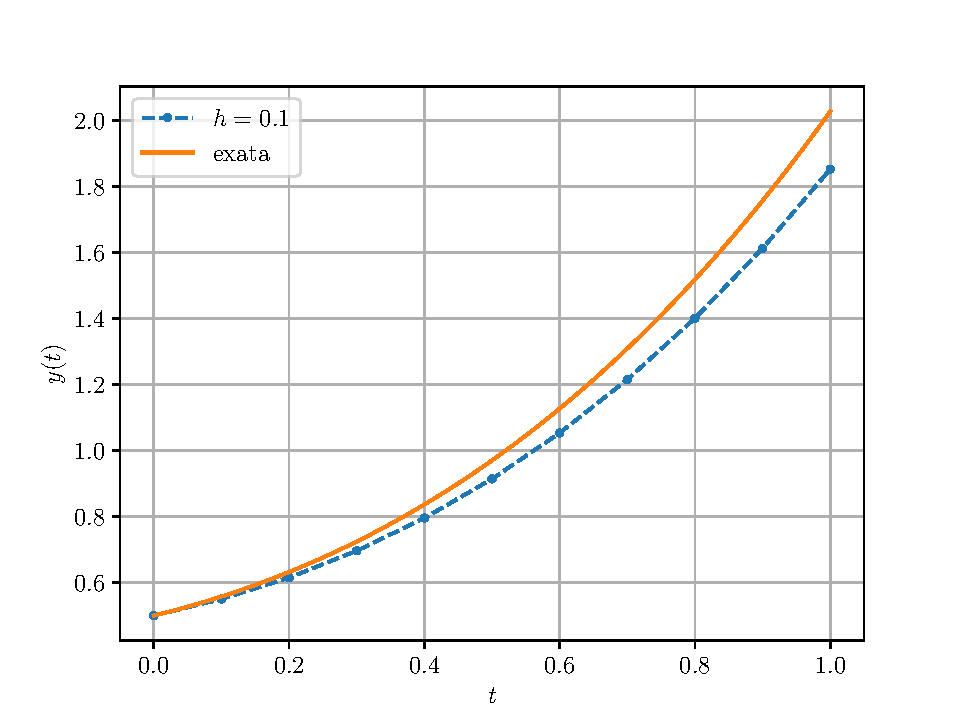
\includegraphics[width=\textwidth]{./cap_pvi/dados/fig_euler_ex0/fig}
  \caption{Esboço das soluções numérica (pontos) e analítica (linha) para o problema do Exemplo~\ref{cap_pvi_sec_euler:ex:euler_ex0}.}
  \label{fig:ex_Euler_1}
\end{figure}
\end{ex}

\begin{lstlisting}[caption=euler.py, label=cap_pvi_sec_euler:cod:euler]
def euler(f, t0, y0, h, n):
    t = np.empty(n+1)
    t[0] = t0
    y = np.empty(n+1)
    y[0] = y0
    for k in range(n):
        t[k+1] = t[k] + h
        y[k+1] = y[k] + h*f(t[k], y[k])
    return t, y
\end{lstlisting}

\subsection{Análise Numérica}

O Método de Euler com passo $h$ aplicado ao problema de valor inicial \eqref{cap_pvi_sec_euler:eq:pvi}, pode ser escrito da seguinte forma
\begin{subequations}\label{cap_pvi_sec_euler:eq:mps}\hleq
  \begin{align}
    \tilde{y}(t^{(0)}; h) &= y_0,\\
    \tilde{y}(t^{(k+1)}; h) &= \tilde{y}(t^{(k)}; h) + h\Phi(t^{(k)}, \tilde{y}(t^{(k)}); h),
  \end{align}
\end{subequations}
onde $\tilde{y}(t^{(k)})$ representa a aproximação da solução exata $y$ no tempo $t^{(k)}=t_0+ kh$, $k=0, 1, 2, \ldots$. Métodos que podem ser escritos dessa forma, são chamados de \hl{\emph{Métodos de Passo Simples}} (ou único). No caso específico do Método de Euler, temos
\begin{equation}\hleq
  \Phi(t, y; h) := f(t, y(t)).
\end{equation}

\subsubsection{Consistência}

Agora, considerando a solução exata $y$ de \eqref{cap_pvi_sec_euler:eq:pvi}, introduzimos
\begin{equation}\hleq
  \Delta(t, y; h) := \left\{
    \begin{array}{ll}
      \displaystyle\frac{y(t+h)-y(t)}{h} &, h\neq 0,\\
      f(t, y(t)) &, h=0.
    \end{array}\right.
\end{equation}

Com isso, vamos analisar o chamado \hl{\emph{erro de discretização local}}
\begin{equation}\hleq
  \tau(t, y; h) := \Delta(t, y; h) - \Phi(t, y; h),
\end{equation}
que \hl{estabelece uma medida quantitativa com que a solução exata $y(t)$ no tempo $t+h$ satisfaz a iteração do método de passo simples}.

\begin{defn}\normalfont{\hl{(Consistência.)}}\label{cap_pvi_sec_euler:defn:consistencia}
  Um \hl{método} de passo simples é dito ser \hl{consistente} quando
  \begin{equation}\hleq
    \lim_{h\to 0}\tau(t,y;h) = 0,
  \end{equation}
  ou, equivalentemente, quando
  \begin{equation}
    \lim_{h\to 0} \Phi(t, y; h) = f(t, y).
  \end{equation}
\end{defn}

\begin{obs}\normalfont{(Consistência do Método de Euler.)}
  Da Definição~\ref{cap_pvi_sec_euler:defn:consistencia}, temos que o \hl{Método de Euler é consistente}. De fato, temos
  \begin{align}
    \lim_{h\to 0} \tau(t, y; h) &= \lim_{h\to 0} \left(\Delta(t, y; h) - \Phi(t, y; h)\right)\\
                                &= \lim_{h\to 0} \left(\frac{y(t+h)-y(t)}{h} - f\left(t,y(t)\right)\right)\\
                                &= y'(t) - f\left(t, y(t)\right) = 0.
  \end{align}
\end{obs}

A \hl{\emph{ordem do erro de discretização local}} de um método de passo simples é dita ser $p$, quando
\begin{equation}\hleq
  \tau(t, y; h) = O(h^p),
\end{equation}
ou seja, quando
\begin{equation}
  \lim_{h\to 0} \frac{\tau(t, y; h)}{h^p} = C,
\end{equation}
para alguma constante $C$.

Para determinarmos a ordem do Método de Euler, tomamos a \hl{expansão em série de Taylor}{\taylor} da solução exata $y(t)$ em torno de $t$, i.e.
\begin{equation}\label{cap_pvi_sec_euler:eq:taylor}
  y(t+h) = y(t) + hy'(t) + \frac{h^2}{2}y''(t) + \frac{h^3}{6}y'''(t+\theta h),
\end{equation}
para algum $0<\theta<1$.
Como $y'(t)=f(t, y(t))$, temos
\begin{align}
  y''(t) &= \frac{d}{dt}f(t, y(t)) \\
         &= f_t(t, y) + f_y(t, y)y'\\
         &= f_t(t, y) + f_y(t, y)f(t, y).
\end{align}
Então, rearranjando os termos em \eqref{cap_pvi_sec_euler:eq:taylor}, obtemos
\begin{equation}\label{eq:pvi_delta_aux}
  \Delta(t, y; h) = f(t, y(t)) + \frac{h}{2}[f_t(t, y) + f_y(t, y)f(t, y)] + O(h^2).
\end{equation}
Portanto, para o Método de Euler temos
\begin{align}
  \tau(t, y; h) &:= \Delta(t, y; h)-\Phi(t, y; h)\\
              &= \Delta(t, y; h) - f(t, y)\\
              &= \frac{h}{2}[f_t(t, y) + f_y(t, y)f(t, y)] + O(h^2)\\
              &= O(h).
\end{align}
Isto mostra que o \hl{Método de Euler é de ordem $1$}.

\subsubsection{Convergência}

A análise acima trata apenas da consistência do Método de Euler. Para analisarmos a \hl{convergência} de métodos de passo simples, definimos o \hl{\emph{erro de discretização global}}
\begin{equation}\hleq
  e(t; h_n) := \tilde{y}(t; h_n) - y(t),
\end{equation}
onde $\tilde{y}(t; h_n) \approx y(t)$ para $h_n := (t-t_0)/n$. Dizemos que o método é \hl{\emph{convergente}} quando
\begin{equation}\hleq
  \lim_{n\to \infty} e(t; h_n) = 0.
\end{equation}
Ainda, dizemos que o método tem \hl{erro de discretização global de ordem $p$} quando
\begin{equation}\hleq
  e(t; h_n) = O(h_n^p)
\end{equation}
para todo $t\in [t_0, t_f]$, $t_f > t_0$.

\begin{lema}\normalfont{(\cite[Cap. 7, Seção 7.2]{Stoer1993a})}\label{cap_pvi_sec_euler:lema:aux}
  Se a sequência $\left(\xi^{(k)}\right)_{k\in\mathbb{R}}$ satisfaz a estimativa
  \begin{equation}
    \left|\xi^{(k+1)}\right| \leq (1 + \delta)\left|\xi^{(k)}\right| + B,
  \end{equation}
  para dados $\delta > 0$ e $B\geq 0$, $k=0, 1, 2, \ldots$, então
  \begin{equation}
    \left|\xi^{(n)}\right| \leq e^{n\delta}\left|\xi^{(0)}\right| + \frac{e^{n\delta}-1}{\delta}B.
  \end{equation}
\end{lema}
\begin{dem}
  De forma iterativa, temos
  \begin{align}
    \left|\xi^{(1)}\right| &\leq (1 + \delta)\left|\xi^{(0)}\right| + B\\
    \left|\xi^{(2)}\right| &\leq (1 + \delta)\left|\xi^{(1)}\right| + B\\
                           &= (1+\delta)^2\left|\xi^{(0)}\right| + (1+\delta)B + B\\
                           &\vdots\\
    \left|\xi^{(k)}\right| &\leq (1 + \delta)^k\left|\xi^{(0)}\right| + B\sum_{k=0}^{k-1}(1+\delta)^k\\
                           &= (1 + \delta)^k\left|\xi^{(0)}\right| + B\frac{(1+\delta)^k-1}{\delta}.
  \end{align}
  Observando que $0<1+\delta\leq e^{\delta}$ para $\delta>-1$, concluímos que
  \begin{equation}
    \left|\xi^{(k)}\right| \leq e^{k\delta}\left|\xi^{(0)}\right| + \frac{e^{k\delta}-1}{\delta}B.
  \end{equation}
\end{dem}

\begin{teo}\normalfont{\hl{(Estimativa do Error Global.)}}\label{cap_pvi_sec_euler:teo:conv}
  Considere o PVI \eqref{cap_pvi_sec_euler:eq:pvi}, para $t_0 = a$, $y_0\in\mathbb{R}$. Suponha que $f$ é Lipschitz contínua em $y$
  \begin{equation}
    |f(t, y) - f(t, z)| \leq L|y - z|,
  \end{equation}
  para todo $(t,y)\in [a, b]\times\mathbb{R}$ e que exista $M>0$ tal que
  \begin{equation}
    |y''(t)| \leq M,
  \end{equation}
  para todo $t\in [a, b]$. Então, as iteradas do Método de Euler $y^{(k)} \approx y\left(t^{(k)}\right)$, $t^{(k)} = t_0 + kh$, $h > (b-a)/n$, $k=0, 1, 2, \dotsc, n+1$, satisfazem a seguinte \hl{\emph{estimativa do erro de discretização global}}
  \begin{equation}\label{cap_pvi_sec_euler:eq:est_errg}\hleq
    \left|y^{(k)} - y\left(t^{(k)}\right)\right| \leq \frac{hM}{2L}\left[e^{L\left(t^{(k)}-t_0\right)}-1\right].
  \end{equation}
\end{teo}
\begin{dem}
  Para $k=0$ o resultado é imediato. Agora, usamos o polinômio de Taylor
  \begin{equation}
    y\left(t^{(k+1)}\right) = y\left(t^{(k)}\right) + hf\left(t^{(k)}, y\left(t^{(k)}\right)\right) + \frac{h^2}{2}y''\left(\xi^{(k)}\right),
  \end{equation}
  onde $t^{(k)} \leq \xi^{(k)} \leq t^{(k+1)}$, $k=0, 1, 2, \ldots, n$. Já, as iteradas de Euler são
  \begin{equation}
    y^{(k+1)} = y^{(k)} + hf\left(t^{(k)}, y^{(k)}\right).
  \end{equation}
  Subtraindo esses equações, obtemos
  \begin{equation}
    \begin{aligned}
      y^{(k+1)} - y\left(t^{(k+1)}\right) &= y^{(k)} - y\left(t^{(k)}\right) \\
      &+ h\left[f\left(t^{(k)}, y^{(k)}\right) - f\left(t^{(k)}, y\left(t^{(k)}\right)\right)\right] - \frac{h^2}{2}y''\left(\xi^{(k)}\right)
    \end{aligned}
  \end{equation}
  Da hipótese de $f$ Lipschitz, temos
  \begin{equation}
    \begin{aligned}
      \left|y^{(k+1)} - y\left(t^{(k+1)}\right)\right| &\leq \left|y^{(k)} - y\left(t^{(k)}\right)\right| \\
      &+ hL\left|y^{(k)} - y\left(t^{(k)}\right)\right| + \frac{h^2}{2}\left|y''\left(\xi^{(k)}\right)\right|
    \end{aligned}
  \end{equation}
  Ou, ainda,
  \begin{equation}
    \left|y^{(k+1)} - y\left(t^{(k+1)}\right)\right| \leq (1 + hL)\left|y^{(k+1)} - y\left(t^{(k+1)}\right)\right| + \frac{h^2M}{2}.
  \end{equation}
  Do Lema \ref{cap_pvi_sec_euler:lema:aux}, temos
  \begin{equation}
    \left|y^{(k+1)} - y\left(t^{(k+1)}\right)\right| \leq \frac{h^2M}{2}\frac{e^{khL}-1}{hL},
  \end{equation}
  donde segue a estimativa do erro global \eqref{cap_pvi_sec_euler:eq:est_errg}.
\end{dem}

\begin{obs}\normalfont{\hl{(Convergência.)}}
  Do Teorema \ref{cap_pvi_sec_euler:teo:conv}, \hl{a ordem do erro de discretização global de um método de passo simples é igual a sua ordem do erro de discretização local}. Portanto, o \hl{Método de Euler é convergente e é de ordem $1$}.
\end{obs}

\begin{ex}\label{cap_pvi_sec_euler:ex:conv}
  Consideramos o seguinte problema de valor inicial
  \begin{subequations}
    \begin{align}
      &y' = y + 1, 0 < t < 1,\\
      &y(0) = 0.
    \end{align}
\end{subequations}
  Na Tabela~\ref{cap_pvi_sec_euler:tab:euler_conv}, temos as aproximações $\tilde{y}(1)$ de $y(1)$ computadas pelo Método de Euler com diferentes passos $h$. A solução analítica deste problema é $y(t) = e^{t}-1$.
 
  \begin{table}[h!]
    \centering
    \caption{Resultados referentes ao Exemplo~\ref{cap_pvi_sec_euler:ex:conv}.}
    \begin{tabular}{l|cc}
      $h$ & $\tilde{y}(1)$ & $|\tilde{y}(1)-y(1)|$\\\hline
      $10^{-1}$ & $1.59374$ & $1.2\E-1$ \\
      $10^{-2}$ & $1.70481$ & $1.3\E-2$ \\
      $10^{-3}$ & $1.71692$ & $1.4\E-3$ \\
      $10^{-5}$ & $1.71827$ & $1.4\E-5$ \\
      $10^{-7}$ & $1.71828$ & $1.4\E-7$ \\
      $10^{-9}$ & $1.71828$ & $1.4\E-9$ \\\hline
    \end{tabular}
    \label{cap_pvi_sec_euler:tab:euler_conv}
  \end{table}
\end{ex}

\subsubsection{Erros de Arredondamento}

O Teorema \ref{cap_pvi_sec_euler:teo:conv} não leva em consideração os erros de arredondamento. Levando em conta esses erros, a iteração do Método de Euler tem a forma
\begin{subequations}\label{cap_pvi_sec_euler:eq:euler_errarr}
  \begin{align}
    &\tilde{y}^{(0)} = y_0 + \delta^{(k)},\\
    &\tilde{y}^{(k+1)} = \tilde{y}^{(k)} + hf\left(t^{(k)}, \tilde{y}^{(k)}\right) + \delta^{(k+1)},
  \end{align}
\end{subequations}
onde $\delta^{(k)}$ é o erro devido a arredondamentos na $k$-ésima iterada, $t^{(k)} = t_0 + hk$, $k=0, 1, 2, \dotsc, n$. Assumindo as hipóteses do Teorema \ref{cap_pvi_sec_euler:teo:conv}, podemos mostrar a seguinte estimativa de erro global
\begin{equation}\label{cap_pvi_sec_euler:eq:euler_errarr_est}\hleq
  \begin{aligned}
    \left|\tilde{y}^{(k+1)} - y\left(t^{(k+1)}\right)\right| &\leq \frac{1}{L}\left(\frac{hM}{2} + \frac{\delta}{h}\right)\left[e^{L\left(t^{(k)}-t_0\right)}-1\right]\\
    &+ |\delta_0|e^{L\left(t^{(k)}-t_0\right)},
\end{aligned}
\end{equation}
para $\delta^{(k)} < \delta$, $k=0, 1, 2, \dotsc, n$.

\subsection{Sistemas de Equações}

Seja um \hl{sistema de EDOs\footnote{Equações Diferenciais Ordinárias} com valor iniciais}
\begin{subequations}\label{cap_pvi_sec_euler:eq:sistem}
  \begin{align}
    &\pmb{y}' = \pmb{f}(t, \pmb{y}), t_0 < t \leq t_f,\\
    &\pmb{y}(t_0) = \pmb{y}_0,
  \end{align}
\end{subequations}
com dada $\pmb{f}:(t, \pmb{y})\in [t_0, t_f]\times\mathbb{R}^m\mapsto \mathbb{R}^m$, dados valores iniciais $\pmb{y}_0\in\mathbb{R}^m$ e incógnita $\pmb{y}:t\in [t_0, t_f]\mapsto \mathbb{R}^m$, $n\geq 1$.

Do ponto de vista algorítmico, a \hl{iteração do Método de Euler} é diretamente estendida \hl{para sistemas}:
\begin{equation}
  \begin{aligned}
    &\pmb{y}^{(0)} = \pmb{y}_0,\\
    &\pmb{y}^{(k+1)} = \pmb{y}^{(k)} + h\pmb{f}\left(t^{(k)}, \pmb{y}^{(k)}\right),
  \end{aligned}
\end{equation}
para $\pmb{y}^{(k)}\approx \pmb{y}\left(t^{(k)}\right)$, $t^{(k)} = t_0 + kh$, $h = (t_f-t_0)/n$, $k = 0, 1, 2, \dotsc, n$.

\begin{ex}\label{cap_pvi_sec_euler:ex:sis}
  Consideramos o sistema de EDOs
  \begin{subequations}
    \begin{align}
      &y_1' = -y_1 + y_2 - e^{-t} - \sen(t) + \cos(t),\\
      &y_2' = 2y_1 + 3y_2 - 6e^{t} - 2\cos(t),
    \end{align}
  \end{subequations}
  para $0 < t \leq 1$ com condições iniciais
  \begin{subequations}
    \begin{align}
      &y_1(0) = 0,\\
      &y_2(0) = 3.
    \end{align}
  \end{subequations}
  Este sistema tem solução analítica
  \begin{subequations}
    \begin{align}
      &y_1(t) = e^t - 2e^{-t} + \cos(t),\\
      &y_2(t) = 2e^t + e^{-t}.
    \end{align}
  \end{subequations}
  
  Podemos reescrevê-lo na forma vetorial
  \begin{subequations}
    \begin{align}
      &\underbrace{\begin{bmatrix}
        y_1'\\
        y_2'
      \end{bmatrix}}_{\pmb{y'}(t)} =
      \underbrace{\begin{bmatrix}
        -y_1 + y_2 + e^{-t} - \sen(t) + \cos(t)\\
        2y_1 + 3y_2 - 6e^{t} - 2\cos(t)
      \end{bmatrix}}_{\pmb{f}(t, \pmb{y})}, 0 < t \leq t_f\\
      &\underbrace{\begin{bmatrix}
        y_1(0)\\
        y_2(0)
      \end{bmatrix}}_{\pmb{y}(0)} =
      \underbrace{\begin{bmatrix}
        0\\
        3
      \end{bmatrix}}_{\pmb{y}_0}
    \end{align}
  \end{subequations}

  Usando o Método de Euler com $h=10^{-2}$ obtemos as soluções mostradas na figura abaixo.

  \begin{figure}[H]
    \centering
    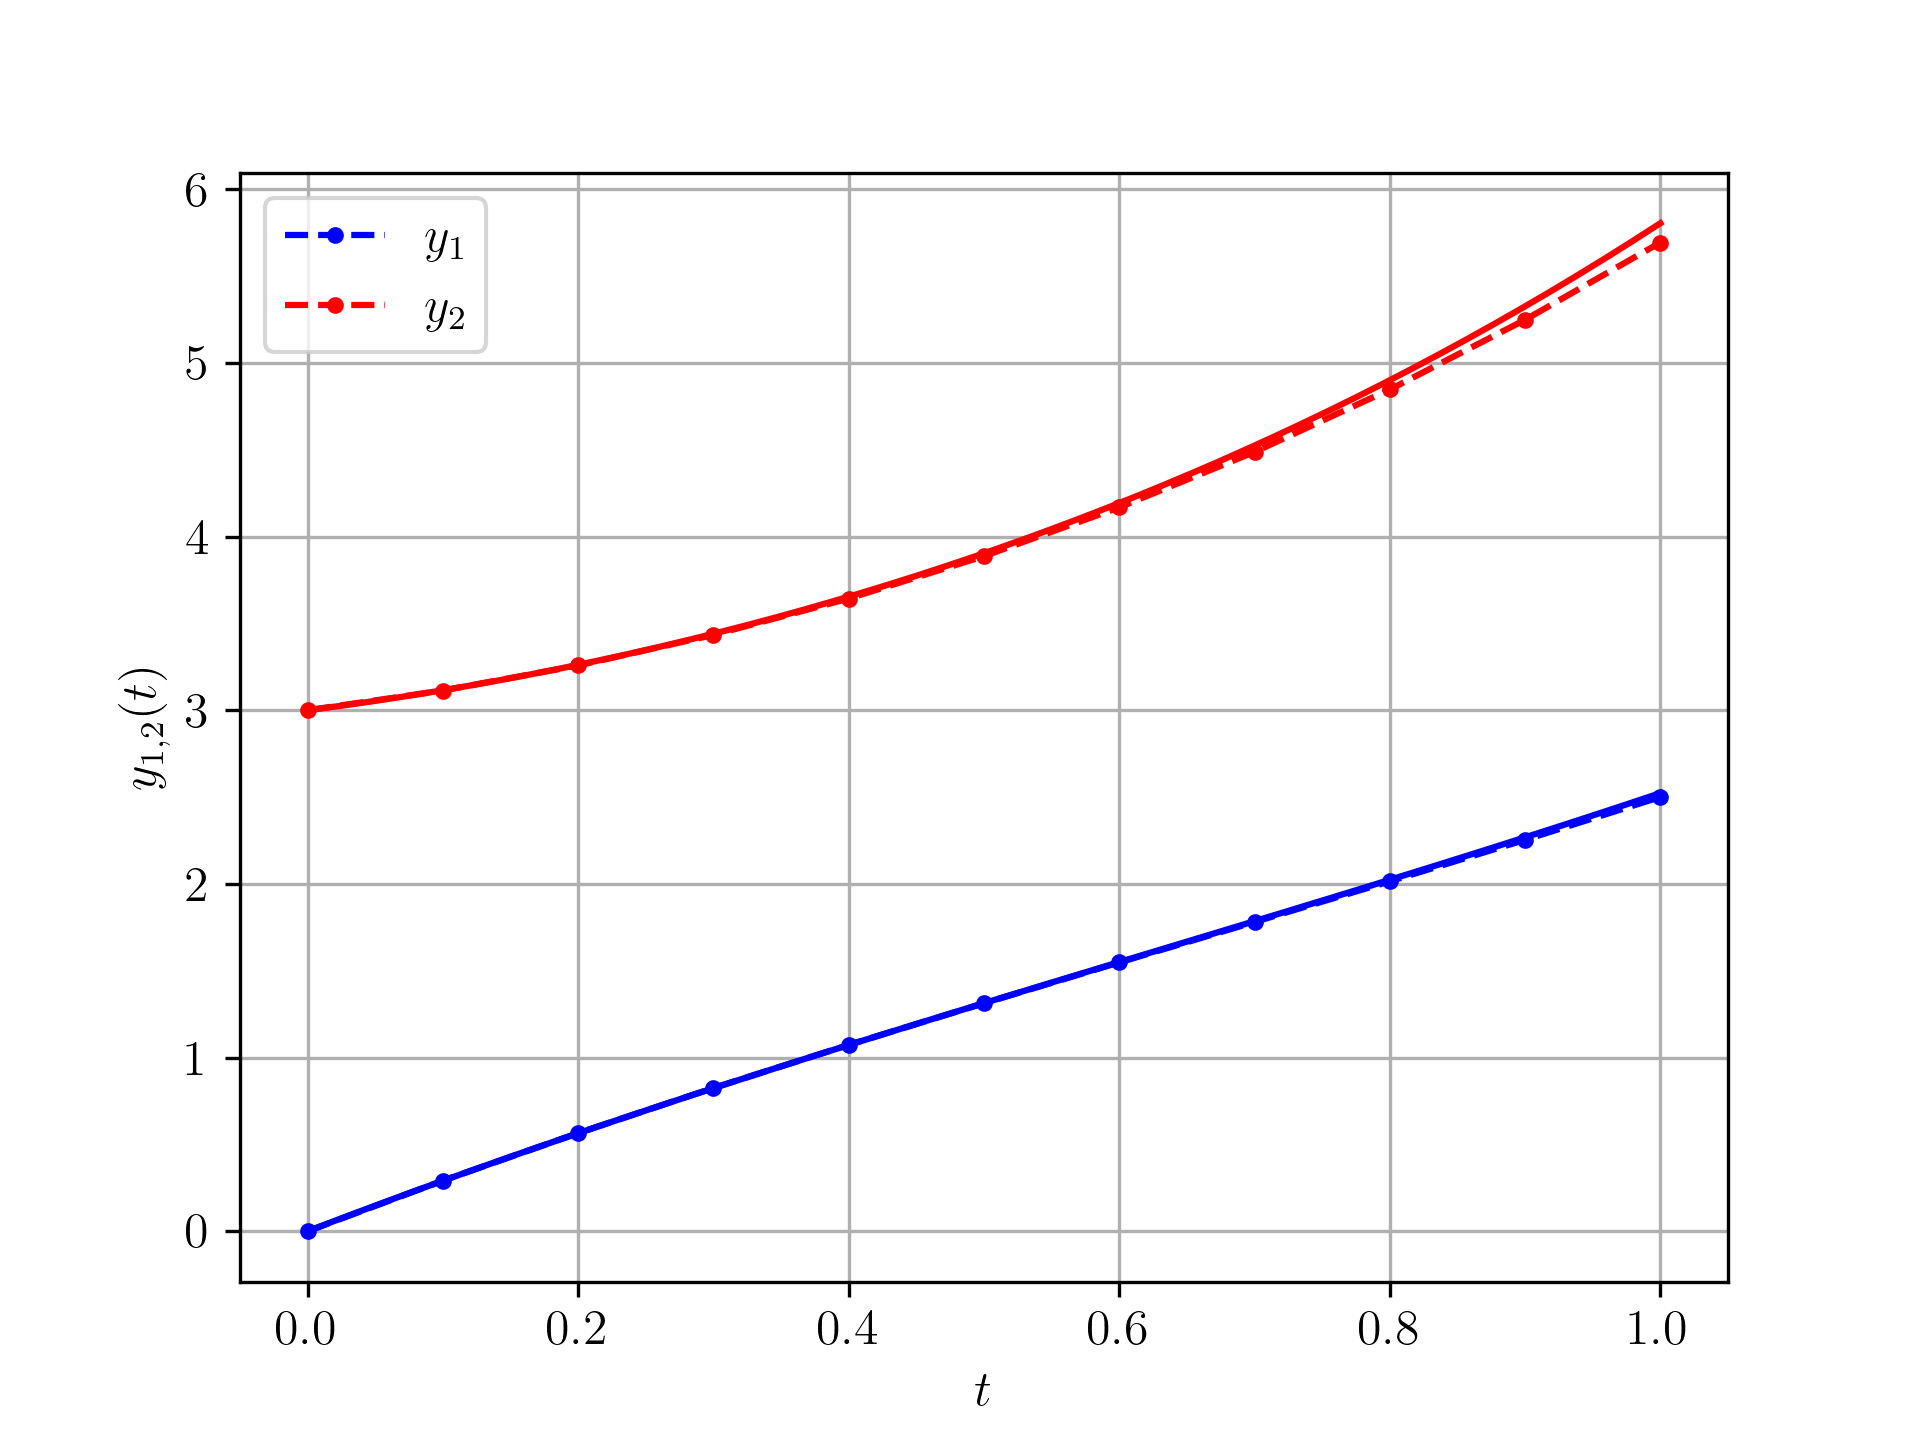
\includegraphics[width=0.8\textwidth]{./cap_pvi/dados/fig_euler_sis/fig}
    \caption{Soluçoes numérica (linha pontilhada) \textit{versus} analítica (linha contínua) para o PVI do Exemplo \ref{cap_pvi_sec_euler:ex:sis}.}
    \label{cap_pvi_sec_euler:fig:sis}
  \end{figure}

\begin{lstlisting}
import numpy as np

def euler(f, t0, y0, h, n):
    t = np.empty(n+1)
    m = y0.size
    y = np.empty((n+1, m))

    t[0] = t0
    y[0] = y0

    for k in range(n):
        t[k+1] = t[k] + h
        y[k+1] = y[k] + h*f(t[k], y[k])
    return t, y

def f(t, y):
    v = np.array([-y[0] + y[1] \
                  - np.exp(-t) \
                  + np.cos(t) \
                  - np.sin(t), \
                  2*y[0] + 3*y[1]
                  - 6*np.exp(t)
                  - 2*np.cos(t)])
    return v


h = 1e-2
n = round(1./h)
t0 = 0.
y0 = np.array([0., 3.])
t,y = euler(f, t0, y0, h, n)
\end{lstlisting}
\end{ex}

\subsection{Equações de Ordem Superior}

Seja dado o PVI de ordem $m$
\begin{subequations}\label{cap_pvi_euler:eq:pvi_ordem_sup}
  \begin{align}
    &\frac{d^m y}{dt^m} = f\left(t, y, \frac{d y}{dt}, \dotsc, \frac{d^{m-1} y}{dt^{m-1}}\right),\\
    &y(t_0) = y_0, \left.\frac{d y}{d t}\right|_{t=0} = y'_0, \dotsc, \left.\frac{d^{(m-1)} y}{d t^{(m-1)}}\right|_{t=0} = y^{(m-1)}_0,
  \end{align}
\end{subequations}
para $t_0 \leq t \leq t_f$.

Para resolvê-lo com o Método de Euler, a ideia é reescrevê-lo como um sistema de EDOs de primeira ordem com condições iniciais. Isso pode ser feito com a mudança de variáveis
\begin{align}
  &u_1 = y,\\
  &u_2 = \frac{d y}{d t},\\
  &u_3 = \frac{d^2 y}{d t^2},\\
  &\qquad\vdots\\
  &u_m = \frac{d^{m-1} y}{d t^{m-1}}.
\end{align}

Com isso e do PVI \eqref{cap_pvi_euler:eq:pvi_ordem_sup}, obtemos o sistema de EDOs de primeira ordem
\begin{subequations}
  \begin{align}
    &u'_1 = u_2,\\
    &u'_2 = u_3,\\
    &u'_3 = u_4,\\
    &\qquad\vdots\\
    &u'_{m} = f(t, u_1, u_2, \dotsc, u_{m}),
  \end{align}
\end{subequations}
para $t_0 < t \leq t_f$ e com condições inicias
\begin{subequations}
  \begin{align}
    &u_1(t_0) = y_0,\\
    &u_2(t_0) = y'_0,\\
    &u_3(t_0) = y''_0,\\
    &\qquad\vdots\\
    &u_{m}(t_0) = y^{(m-1)}_0.
  \end{align}
\end{subequations}

\begin{ex}\label{cap_pvi_sec_euler:ex:pvi_ordemsup}
  Consideramos o seguinte PVI de ordem superior
  \begin{subequations}
    \begin{align}
      &y'' - ty' + y = (2 + t)e^{-t} - t\cos(t), 0 < t \leq 1,\\
      &y(0) = 1, y'(0) = 0.
    \end{align}
  \end{subequations}
  Sua solução analítica é
  \begin{equation}
    y(t) = \sen(t) + e^{-t}.
  \end{equation}

  Para reescrevê-lo como uma sistema de EDOs de primeira ordem, tomamos as mudanças de variáveis $u_1 = y$ e $u_2 = y'$. Com isso, obtemos
  \begin{subequations}
    \begin{align}
      &u'_1 = u_2,\\
      &u_2' = tu_2 - u_1 + (2+t)e^{-t} - t\cos(t),
    \end{align}
  \end{subequations}
  para $0 < t \leq t_f$ e com condições iniciais
  \begin{subequations}
    \begin{align}
      &u_1(0) = 1,\\
      &u_2(0) = 0.
    \end{align}
  \end{subequations}

  Com passo $h=10^{-2}$, o Método de Euler aplicado a este sistema fornece a solução do PVI mostrada na figura abaixo.

  \begin{figure}[H]
    \centering
    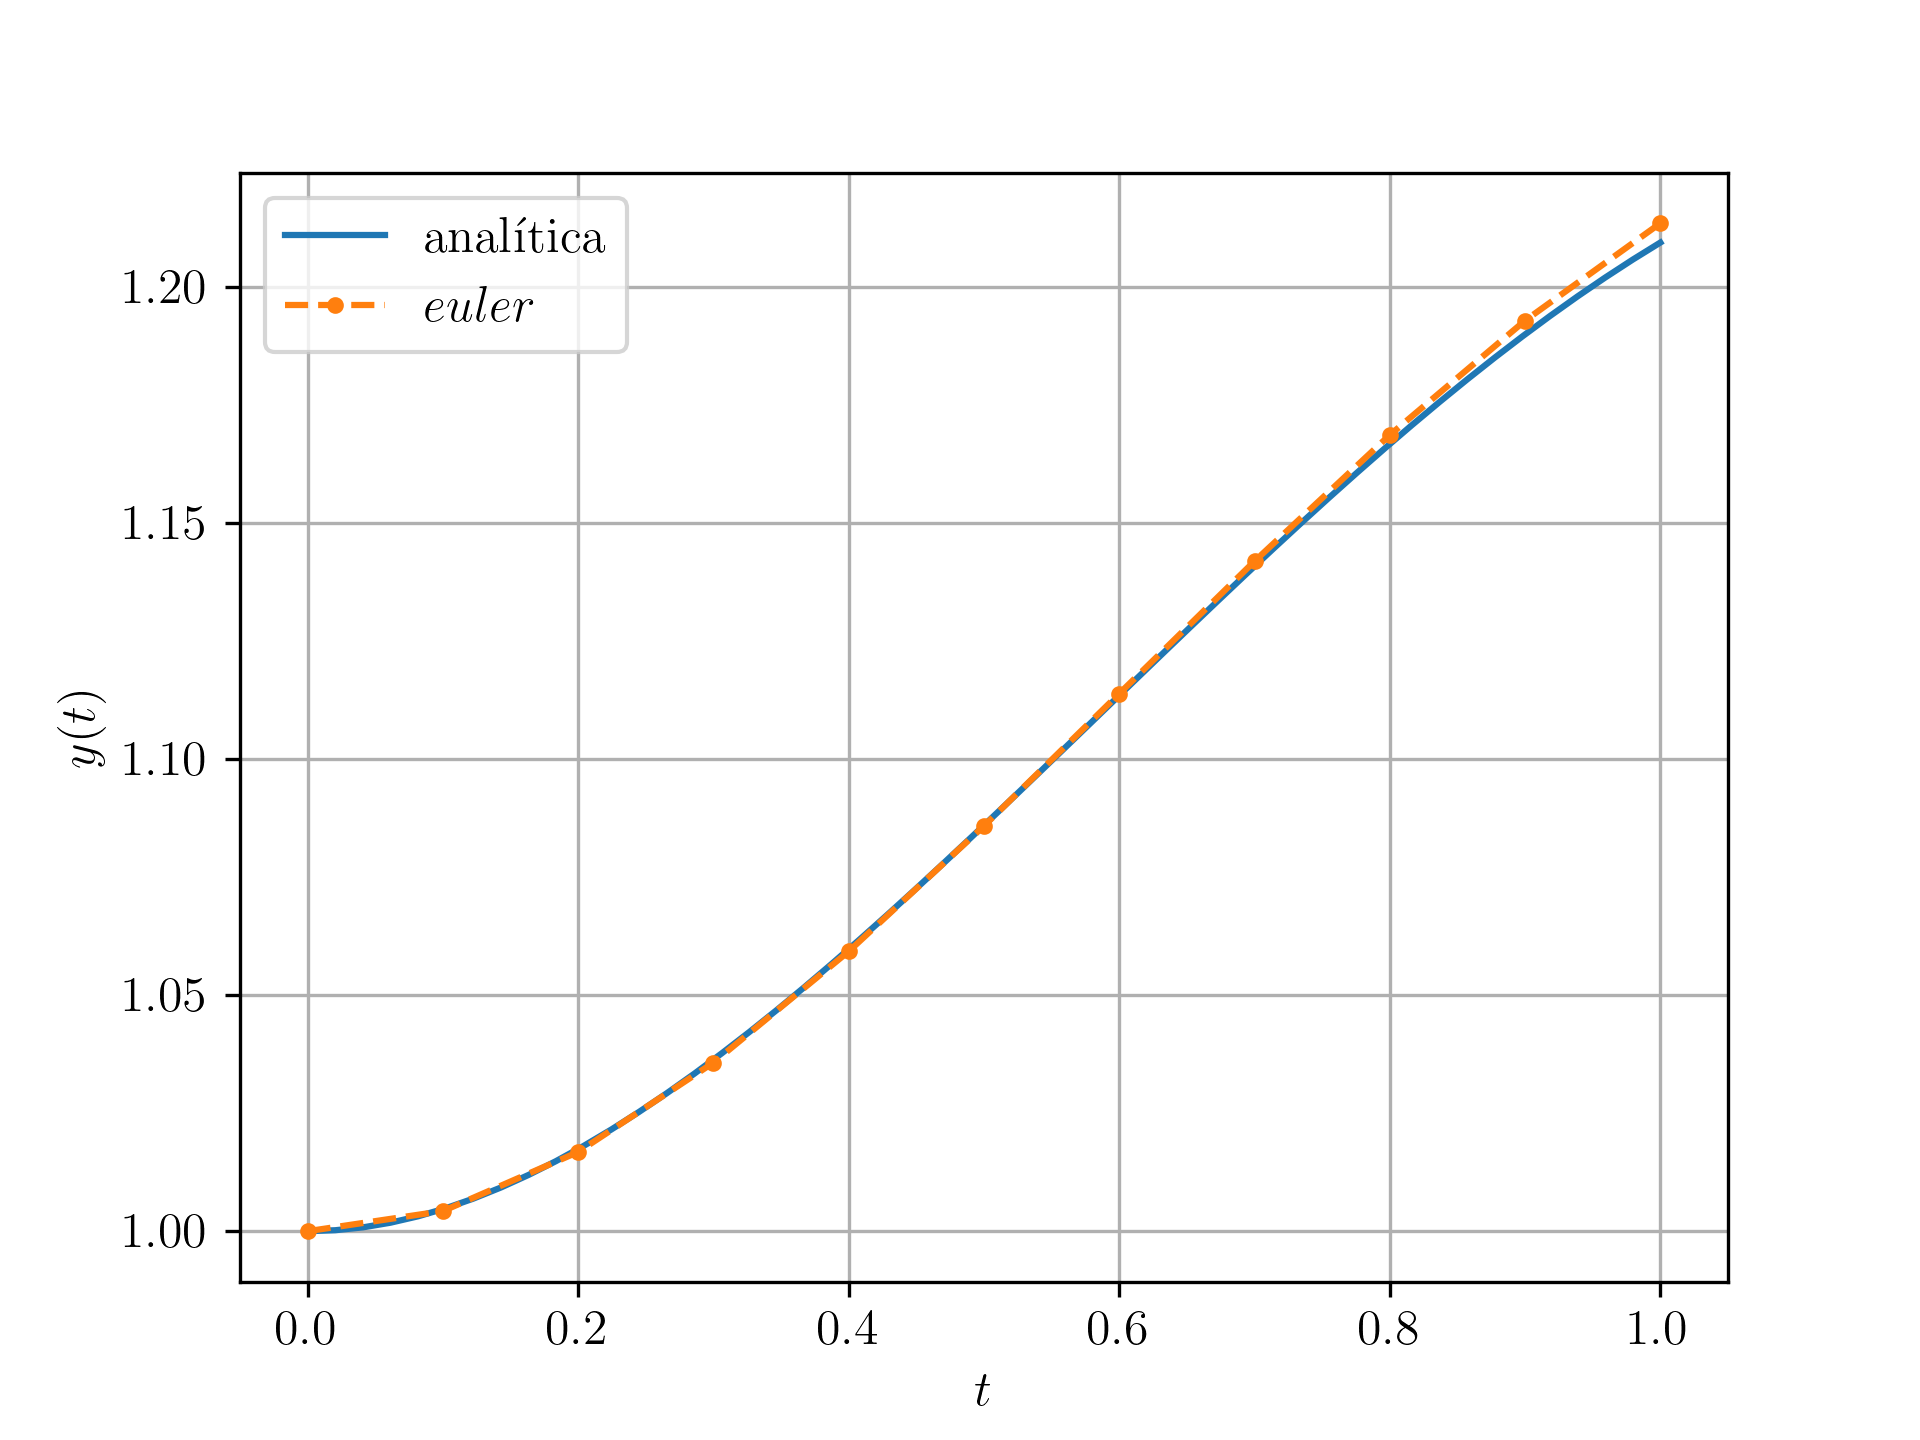
\includegraphics[width=0.8\textwidth]{./cap_pvi/dados/fig_euler_ordemsup/fig}
    \caption{Solução numérica \textit{versus} analítica computadas para o PVI do Exemplo \ref{cap_pvi_sec_euler:ex:pvi_ordemsup}.}
    \label{cap_pvi_sec_euler:fig:pvi_ordemsup}
  \end{figure}
\end{ex}

\subsection{Exercícios}

\begin{exer}
  O problema de valor inicial
  \begin{subequations}
    \begin{align}
      &y' = \pi\left[\cos^2(\pi t) - \sen^2(\pi t)\right], ~0 < t \leq 1.5,\\
      &y(0) = 0.
    \end{align}
  \end{subequations}
  tem solução analítica $y(t) = \sen(\pi t)\cos(\pi t)$. Compute a aproximação $\tilde{y}(1.5; h) \approx y(1.5)$ pelo Método de Euler com passo $h=10^{-1}$ e forneça o erro $e(1.5; h) := \tilde{y}(1.5; h) - y(1.5)$
\end{exer}
\begin{resp}
  $\tilde{y}(1.5) = 3.14159\E-1$, $e(1, h) = 3.1E-01$
\end{resp}

\begin{exer}
  Use o Método de Euler para computar a solução de
  \begin{subequations}
    \begin{align}
      &y' = e^{2t} - 2y,\quad 0 < t\leq 1,\\
      &y(0) = 0.
    \end{align}
  \end{subequations}
  Escolha um passo $h$ adequado de forma que $y(1)$ seja computado com precisão de $5$ dígitos significativos.
\end{exer}
\begin{resp}
  $h=10^{-6}$, $\tilde{y}(1) = 1.8134\E+0$
\end{resp}

\begin{exer}
  Considere o seguinte problema de valor inicial
  \begin{subequations}
    \begin{align}
      &y' + e^{-y^2+1} = 2,\quad t>1,\\
      &y(1) = -1.
    \end{align}
\end{subequations}
Use o Método de Euler para computar o valor aproximado de $y(2)$ com precisão de $6$ dígitos significativos.
\end{exer}
\begin{resp}
  $-5.58858\E-1$
\end{resp}

\begin{exer}
  Use o Método de Euler para computar a solução de
  \begin{subequations}
    \begin{align}
      &y' = -30y,\quad 0 < t\leq 1,\\
      &y(0) = \frac{1}{3}
    \end{align}
  \end{subequations}
  A solução analítica é $y(t) = \frac{1}{3}e^{-30t}$. Compute a solução aproximação $\tilde{y}(1)$ e o erro $|\tilde{y}(1) - y(1)|$ usando o passo $h=10^{-1}$. O erro obtido está de acordo com a estimativa \eqref{cap_pvi_sec_euler:eq:est_errg}?
\end{exer}
\begin{resp}
  $|\tilde{y}(1) - y(1)| = 3.4\E+2$. Dica: verifique as hipóteses do Teorema \ref{cap_pvi_sec_euler:teo:conv}.
\end{resp}

\begin{exer}
  Para o sistema de EDOs do Exemplo \ref{cap_pvi_sec_euler:ex:sis}, verifique a ordem de convergência do Método de Euler computando o erro $\varepsilon = \|\tilde{\pmb{y}}(1) - \pmb{y}(1)\|$ com diferentes tamanhos de passos $h = 10^{-1}, 10^{-2}, \dotsc, 10^{-6}$. 
\end{exer}
\begin{resp}
  \begin{tabular}{l|c|l}
    $h$ & $\tilde{\pmb{y}}(1)$ & $\|\tilde{\pmb{y}}(1) - \pmb{y}(1)\|$ \\\hline
    $10^{-1}$ & $(2.387, 5.077)$ & $7.4\E-1$ \\
    $10^{-2}$ & $(2.500, 5.693)$ & $1.1\E-1$ \\
    $10^{-3}$ & $(2.520, 5.793)$ & $1.2\E-2$ \\
    $10^{-4}$ & $(2.523, 5.803)$ & $1.2\E-3$ \\
    $10^{-5}$ & $(2.523, 5.804)$ & $1.2\E-4$ \\
    $10^{-6}$ & $(2.523, 5.804)$ & $1.2\E-5$ \\\hline
  \end{tabular}
\end{resp}

\begin{exer}
  Para o PVI de segunda ordem dado no Exemplo \ref{cap_pvi_sec_euler:ex:pvi_ordemsup}, tente computar a solução para tempos finais $t_f = 2, 3, \dotsc, 5$. Faça uma comparação gráfica entre as soluções numérica e analítica. O que ocorre ao aumentarmos o tempo final? Justifique sua resposta.
\end{exer}
\begin{resp}
  Dica: O PVI do Exemplo \ref{cap_pvi_sec_euler:ex:pvi_ordemsup} é um problema rígido.
\end{resp}


\subsubsection{Análise Numérica}

\begin{exer}
  Mostre que se $\delta>-1$, então $0 < 1+\delta \leq e^{\delta}$.
\end{exer}
\begin{resp}
  Dica: use o polinômio de Taylor de grau 2 de $e^\delta$.
\end{resp}

\begin{exer}
  Seja dado um PVI \eqref{cap_pvi_sec_euler:eq:pvi}, $t_0\leq t \leq t_f$. Sejam $\tilde{y}^{(k)}$, $k=0, 1, 2, \dotsc, n$, as aproximações computadas conforme em \eqref{cap_pvi_sec_euler:eq:euler_errarr}, com $\delta^{(k)} < \delta$. Assumindo as mesmas hipóteses do Teorema \ref{cap_pvi_sec_euler:teo:conv}, mostre a estimativa de erro global \eqref{cap_pvi_sec_euler:eq:euler_errarr_est}.
\end{exer}
\begin{resp}
  Dica: estude a demonstração do Teorema \ref{cap_pvi_sec_euler:teo:conv}.
\end{resp}

\begin{exer}
  Assumindo um erro de arredondamento máximo de $\delta > 0$, use \eqref{cap_pvi_sec_euler:eq:euler_errarr_est} para obter uma estimativa para a melhor escolha de $h$.
\end{exer}
\begin{resp}
  $h = \sqrt{2\delta/M}$. Dica: Encontre o mínimo de $E(h) := M/2 + \delta/h^2$.
\end{resp}

\section{Métodos de Taylor de Alta Ordem}\label{cap_pvi_sec_taylor}

Métodos de Taylor{\taylor} são usados para computar a solução numérica de Problemas de Valor Inicial (PVI) da forma
\begin{subequations}\label{cap_pvi_sec_taylor:eq:pvi}
  \begin{align}
    &y' = f(t, y),\quad t_0 < t \leq t_f,\\
    &y(t_0) = y_0,
  \end{align}
\end{subequations}
onde $y:[t_0, t_f]\mapsto \mathbb{R}$ é a função incógnita, dada $f:[t_0, t_f]\times\mathbb{R}\to\mathbb{R}$ e dado valor inicial $y_0\in\mathbb{R}$.

Na Seção \ref{cap_pvi_sec_euler}, vimos que \hl{a ordem do erro de discretização local} do Método de Euler{\euler} \hl{é também a do erro de discretização global}. Este resultado é generalizado pelo Teorema \ref{cap_pvi_sec_taylor:teo:conv}, \hl{para todo o método de passo simples}
\begin{subequations}\label{cap_pvi_sec_taylor:eq:iterps}
  \begin{align}
    &y^{(0)} = y_0,\\
    &y^{(k+1)} = y^{(k)} + h\Phi\left(t^{(k)}, y^{(k)}\right),
  \end{align}
\end{subequations}
onde $y^{(k)}\approx y\left(t^{(k)}\right)$, $t^{(k)} = t_0 + kh$, $h = (t_f-t_0)/n$, $k = 0, 1, 2, \dotsc, n$.

Antes, lembramos que o \hl{\emph{erro de discretização local}} é definido por
\begin{equation}\label{cap_pvi_sec_taylor:eq:def_erro_local}\hleq
  \tau(t, y; h) := \Delta(t, y; h) - \Phi(t, y; h),
\end{equation}
onde
\begin{equation}\hleq
  \Delta(t, y; h) := \left\{
    \begin{array}{ll}
      \displaystyle\frac{y(t+h) - y(t)}{h} &, h\neq 0,\\
      f\left(t, y(t)\right) &, h=0.
    \end{array}
  \right.
\end{equation}

Já, o \hl{\emph{erro de discretização global}} é definido por
\begin{equation}\hleq
  e(t; h_n) := \tilde{y}(t; h_n) - y(t),
\end{equation}
onde $\tilde{y}(t; h_n) \approx y(t)$ dada por \eqref{cap_pvi_sec_taylor:eq:iterps} para $h_n = (t-t_0)/n$.

Com o objetivo de desenvolvermos métodos de alta ordem, podemos usar o polinômio de Taylor de ordem $m$ de $y=y(t)$
\begin{equation}
  \begin{aligned}
    y(t+h) &= y(t) + hy'(t) + \frac{h^2}{2}y''(t)\\
    &+ \cdots + \frac{h^m}{m!}\frac{d^m y}{d t^m}(t) + \frac{h^{m+1}}{(m+1)!}\frac{d^{m+1} y}{d t^{m+1}}(\xi),
  \end{aligned}
\end{equation}
donde
\begin{equation}\label{cap_pvi_sec_taylor:eq:y_poli_taylor}
  \begin{aligned}
    y(t+h) &= y(t) + hf(t, y) + \frac{h^2}{2}f'(t, y) \\
    &+ \cdots + \frac{h^m}{m!}\frac{d^{m-1} f}{d t^{m-1}}(t, y) \\
    & + \frac{h^{m+1}}{(m+1)!}\frac{d^{m} f}{d t^{m}}\left(\xi, y(\xi)\right)
  \end{aligned}
\end{equation}
e, portanto
\begin{equation}\label{cap_pvi_sec_taylor:eq:delta_taylor}
  \begin{aligned}
    \Delta(t, y; h) &= f(t, y) + \frac{h}{2}f'(t, y) \\
    &+ \cdots + \frac{h^m}{m!}\frac{d^{m-1} f}{d t^{m-1}}(t, y) \\
    & + \frac{h^{m+1}}{(m+1)!}\frac{d^{m} f}{d t^{m}}\left(\xi, y(\xi)\right)
  \end{aligned}  
\end{equation}

Isto nos motiva a \hl{\emph{iteração do Método de Taylor de Ordem $m$}}:
\begin{subequations}\hleq
  \begin{align}
    &y^{(0)} = y_0,\\
    &y^{(k+1)} = y^{(k)} + hT^{(m)}\left(t^{(k)}, y^{(k)}\right),
  \end{align}  
\end{subequations}
onde
\begin{equation}\hleq
  \begin{aligned}
    T^{(m)}\left(t^{(k)}, y^{(k)}\right) &:= f\left(t^{(k)}, y^{(k)}\right) + \frac{h}{2}f'\left(t^{(k)}, y^{(k)}\right)\\
    &+ \cdots + \frac{h^{m-1}}{m!}\frac{d^{m-1} f}{d t^{m-1}}\left(t^{(k)}, y^{(k)}\right)
\end{aligned}
\end{equation}

\begin{ex}
  Considere o PVI
  \begin{subequations}
    \begin{align}
      &y' = y + \sen(t),\quad 0 < t \leq 1,\\
      &y(0) = \frac{1}{2}.
    \end{align}
  \end{subequations}
  Vamos usar o Método de Taylor de Ordem 2 para computar sua solução e comparar com a solução analítica
  \begin{equation}
    y(t) = e^t - \frac{1}{2}\sen(t) - \frac{1}{2}\cos(t).
  \end{equation}

  \begin{center}
    \begin{tabular}[H]{ll}
      $h$ & $\left|\tilde{y}(1) - y(1)\right|$\\\hline
      $10^{-1}$ & $4.9\E-3$ \\
      $10^{-2}$ & $5.2\E-5$ \\
      $10^{-3}$ & $5.2\E-7$ \\
      $10^{-4}$ & $5.2\E-9$ \\
      $10^{-5}$ & $5.2\E-11$ \\\hline
    \end{tabular}
  \end{center}

\begin{lstlisting}[caption=taylor.py, label=cap_pvi_sec_taylor:cod:taylor.py]
import numpy as np

def taylor(Phi, t0, y0, h, n):
    t = t0
    y = y0
    for k in range(n):
        y += h*Phi(t, y, h)
        t += h
    return t, y

def f(t, y):
    return y + np.sin(t)

def fl(t, y):
    return f(t, y) + np.cos(t)

def Phi(t, y, h):
    return f(t, y) + h/2*fl(t, y)

# analítica
def exata(t):
    return np.exp(t) - 0.5*np.sin(t) - 0.5*np.cos(t)

h = 1e-1
n = round(1/h)
t,y = taylor(Phi, 0., 0.5, h, n)
\end{lstlisting}
\end{ex}

\subsection{Análise Numérica}

\begin{teo}\normalfont{(\hl{Convergência}, \cite[Cap. 7, Seção 7.2]{Stoer1993a}.)}\label{cap_pvi_sec_taylor:teo:conv}
  Considere o PVI \eqref{cap_pvi_sec_taylor:eq:pvi}, para $t_0\in [a, b]$ e $y_0\in\mathbb{R}$. Seja $\Phi$ contínua em
  \begin{equation}
    G := \{(t, y, h): a\leq t\leq b, |y-y(t)|\leq\gamma, 0\leq|h|\leq h_0\},
  \end{equation}
  para $h_0>0$ e $\gamma>0$. Sejam também, $M, N$ constantes tais que
  \begin{equation}
    \left|\Phi(t, y; h) - \Phi(t, z; h)\right| \leq M|y - z|,
  \end{equation}
  para todas $(t, y; h), (t, z; h)\in G$. Se, ainda, para algum $p>0$ e para todo $t\in [a, b]$, $|h|\leq h_0$, temos a \hl{\emph{estimativa do erro de discretização local}}
  \begin{equation}\label{cap_pvi_sec_taylor:eq:est_erro_local}\hleq
    \left|\tau(t, y(t); h)\right| \leq N |h|^p,
  \end{equation}
  então existe $\overline{h}$, $0<\overline{h}<h_0$, tal que vale a seguinte \hl{\emph{estimativa do erro de discretização global}}
  \begin{equation}\label{cap_pvi_sec_taylor:eq:est_erro_global}\hleq
    |e(t; h_n)| \leq |h_n|^pN\frac{e^{M|t-t_0|}-1}{M},
  \end{equation}
  para todo $t\in [a, b]$ e para todo $h_n = (t-t_0)/n$, $n=1, 2, \ldots$, com $|h_n|\leq \overline{h}$.
\end{teo}
\begin{dem}
  Seja
  \begin{equation}
    \tilde{\Phi}(t, y; h) := \left\{
      \begin{array}{ll}
        \Phi(t, y; h) &, (t, y, h)\in G,\\
        \Phi(t, y(t)+\gamma; h) &, t\in [a, b], |h|\leq h_0, y\geq y(t)+\gamma,\\
        \Phi(t, y(t)-\gamma; h) &, t\in [a, b], |h|\leq h_0, y\leq y(t)-\gamma,
      \end{array}
    \right.
  \end{equation}
  A função $\tilde{\Phi}$ é contínua em
  \begin{equation}
    \tilde{G} := \{(t, y; h): t\in [a, b], y\in\mathbb{R}, |h|\geq h_0\}
  \end{equation}
  e satisfaz
  \begin{equation}\label{cap_pvi_sec_taylor:eq:aux0}
    \left|\tilde{\Phi}(t, y; h) - \tilde{\Phi}(t, z; h)\right| \leq M|y - z|,
  \end{equation}
  para todas $(t, y; h), (t, z; h)\in \tilde{G}$. Ainda, como $\tilde{\Phi}(t, y(t); h) = \Phi(t, y(t); h)$, também temos que
  \begin{equation}\label{cap_pvi_sec_taylor:eq:aux1}
    |\Delta(t, y(t); h) - \tilde{\Phi}(t, y(t); h)| \leq N |h|^p,
  \end{equation}
  para $t\in [a, b]$ e $|h|\leq h_0$.

  Sejam, $\tilde{y}^{(k)} := \tilde{y}\left(t^{(k)}; h\right)$, $t^{(k)} = t_0 + kh$, $\tilde{y}^{(0)} = y_0$:
  \begin{align}
    \tilde{y}^{(k+1)} = \tilde{y}^{(k)} + h\tilde{\Phi}\left(t^{(k)}, \tilde{y}^{(k)}; h\right),
    y\left(t^{(k+1)}\right) = y\left(t^{(k)}\right) + h\Delta\left(t^{(k)}, y\left(t^{(k)}\right); h\right).
  \end{align}
  Definindo $\tilde{e}^{(k)} := \tilde{y}^{(k)} - y\left(t^{(k)}\right)$, obtemos a fórmula de recorrência
  \begin{align}
    \tilde{e}^{(k+1)} &= \tilde{e}^{(k)} + h\left[\tilde{\Phi}\left(t^{(k)}, \tilde{y}^{(k)}; h\right) - \Delta\left(t^{(k)}, y\left(t^{(k)}\right); h\right)\right]\\
                      &= \tilde{e}^{(k)} + h\left[\tilde{\Phi}\left(t^{(k)}, \tilde{y}^{(k)}; h\right) - \tilde{\Phi}\left(t^{(k)}, y\left(t^{(k)}\right); h\right)\right]\\
                      &+ h\left[\tilde{\Phi}\left(t^{(k)}, y\left(t^{(k)}\right); h\right) - \Delta\left(t^{(k)}, y\left(t^{(k)}\right); h\right)\right].\label{cap_pvi_sec_taylor:eq:aux2}
  \end{align}
  Agora, de \eqref{cap_pvi_sec_taylor:eq:aux0} e \eqref{cap_pvi_sec_taylor:eq:aux1}, temos
  \begin{align}
    &\left|\tilde{\Phi}\left(t^{(k)}, \tilde{y}^{(k)}; h\right) - \tilde{\Phi}\left(t^{(k)}, y\left(t^{(k)}\right); h\right)\right| \leq M\left|\tilde{e}^{(k)}\right|\\
    &\left|\Delta\left(t^{(k)}, y\left(t^{(k)}\right); h\right) - \tilde{\Phi}\left(t^{(k)}, y\left(t^{(k)}\right); h\right)\right| \leq N |h|^p
  \end{align}
  Portanto, de \eqref{cap_pvi_sec_taylor:eq:aux2}, temos
  \begin{equation}
    \left|\tilde{e}^{(k+1)}\right| \leq \left(1 + |h|M\right)\left|\tilde{e}^{(k)}\right| + N |h|^{p+1}
  \end{equation}
  Então, do Lema \ref{cap_pvi_sec_euler:lema:aux}, temos
  \begin{equation}\label{cap_pvi_sec_taylor:eq:aux3}
    \left|\tilde{e}^{(k)}\right| \leq N|h|^p\frac{e^{k|h|M}-1}{M}.
  \end{equation}
  Sejam, agora, $t\in [a, b]$, $t\neq t_0$ fixo e $h := h_n = (t-t_0)/n$, $n>0$. Então, $t^{(n)} = t_0 + nh = t$ e de \eqref{cap_pvi_sec_taylor:eq:aux3} temos
  \begin{equation}
    \left|\tilde{e}\left(t, h_n\right)\right| \leq N|h_n|^p\frac{e^{M|t-t_0|}-1}{M},
  \end{equation}
  para todo $t\in [a, b]$, $|h_n|\leq h_0$. Uma vez que $|t-t_0|\leq |b-a|$ e $\gamma >0$, existe $\overline{h}$, $0<\overline{h}\leq h_0$, tal que $\left|\tilde{e}\left(t, h_n\right)\right| \leq \gamma$ para todo $t\in [a, b]$ e $|h_n|\leq \overline{h}$. Logo, para o método de passo simples \eqref{cap_pvi_sec_taylor:eq:iterps} gerado por $\Phi$, temos para $|h|\leq\overline{h}$ que
  \begin{align}
    &\tilde{y}^{(k)} = y^{(k)},\\
    &\tilde{e}^{(k)} = e^{(k)},\\
    &\tilde{\Phi}\left(t^{(k)}, \tilde{y}^{(k)}; h\right) = \Phi\left(t^{(k)}, \tilde{y}^{(k)}; h\right).
  \end{align}
  Concluímos que
  \begin{equation}
    \left|e\left(t, h_n\right)\right| \leq N|h_n|^p\frac{e^{M|t-t_0|}-1}{M},
  \end{equation}
  para todo $t\in [a, b]$ e $h_n = (t-t_0)/n$, $n=1, 2, \ldots$, com $|h_n|\leq \overline{h}$.
\end{dem}

\subsection{Exercícios}

\begin{exer}
  Use o Método de Taylor de $O(h^2)$ para computar a solução de
  \begin{subequations}\label{cap_pvi_sec_taylor:eq:pvi_exer_0}
    \begin{align}
      &y' + \cos(t) = y,\quad 0 < t \leq 1,\\
      &y(0) = \frac{1}{2}.
    \end{align}
  \end{subequations}
  A solução analítica é $y(t) = \frac{1}{2}\cos(t) - \frac{1}{2}\sin(t)$. Faça testes numéricos com $h=10^{-1}$, $10^{-2}$, $10^{-3}$ e $10^{-4}$, observe os resultados obtidos e o erro $\varepsilon := |\tilde{y}(1) - y(1)|$, onde $\tilde{y}$ corresponde a solução numérica. O erro tem o comportamento esperado? Justifique sua resposta.
\end{exer}
\begin{resp}
  \begin{tabular}{c|c|c}
    $h$ & $\tilde{y}(1)$ & $\left|\tilde{y}(1)-y(1)\right|$\\\hline
    $1\E-1$ & $-1.52293\E-1$ & $1.7\E-3$ \\
    $1\E-2$ & $-1.50602\E-1$ & $1.8\E-5$ \\
    $1\E-3$ & $-1.50585\E-1$ & $1.8\E-7$ \\
    $1\E-4$ & $-1.50584\E-1$ & $1.8\E-9$ \\\hline
  \end{tabular}
\end{resp}

\begin{exer}
  Use o Método de Taylor $O(h^2)$ para computar a solução do PVI \eqref{cap_pvi_sec_taylor:eq:pvi_exer_0} com $h=10^{-1}$. Faça um esboço do gráfico do erro $e\left(t; h=10^{-1}\right) = \left|\tilde{y}(t) - y(t)\right|$ e verifique se ele tem a forma esperada conforme a estimativa do erro global \eqref{cap_pvi_sec_taylor:eq:est_erro_global}.
\end{exer}
\begin{resp}
  Dica: o gráfico de $e\left(t; h=10^{-1}\right)$ tem a forma de uma função exponencial crescente.
\end{resp}

\begin{exer}
  Use o Método de Taylor de $O(h^3)$ para computar a solução do PVI \eqref{cap_pvi_sec_taylor:eq:pvi_exer_0}. Escolha o passo $h$ de forma que a solução numérica tenha precisão de 6 dígitos significativos.
\end{exer}
\begin{resp}
  $h=10^{-2}$, $\tilde{y}(1) = -1.50584\E-1$
\end{resp}

\begin{exer}
  Considere o seguinte PVI
  \begin{subequations}
    \begin{align}
      &y' = y^2 - ty,\quad 1 < t \leq 2,\\
      &y(1) = -2.
    \end{align}
  \end{subequations}
  Compute a solução com o Método de Taylor de $O\left(h^p\right)$ com passo $h = 10^{-1}$:
  \begin{enumerate}[a)]
  \item $p = 2$.
  \item $p = 3$.
  \item $p = 4$.
  \end{enumerate}
\end{exer}
\begin{resp}
  Dica: $y(2) = -2.10171\E-1$.
\end{resp}

\begin{exer}
  Considere o seguinte PVI
  \begin{subequations}
    \begin{align}
      &y' - t^2y = 0,\quad 1 < t \leq 3,\\
      &y(1) = \frac{1}{2}.
    \end{align}
  \end{subequations}
  Compute a solução com o Método de Taylor de $O\left(h^p\right)$ com passo $h = 10^{-1}$:
  \begin{enumerate}[a)]
  \item $p = 2$.
  \item $p = 3$.
  \item $p = 4$.
  \end{enumerate}
\end{exer}
\begin{resp}
  Dica: $y(2) = 2.90306\E+3$.
\end{resp}

\subsubsection{Análise Numérica}

\begin{exer}
  Considere o PVI \eqref{cap_pvi_sec_taylor:eq:pvi_exer_0}. Verifique que o Método de Taylor de $O(h^2)$ satisfaz as estimativas do erro local \eqref{cap_pvi_sec_taylor:eq:est_erro_local} e do erro global \eqref{cap_pvi_sec_taylor:eq:est_erro_global}. Forneça valor estimados para os parâmetros $N$ e $M$.
\end{exer}


\section{Métodos de Runge-Kutta}\label{cap_pvi_sec_rk}

Seja um Problema de Valor Inicial (PVI) da forma
\begin{subequations}\label{cap_pvi_sec_rk:eq:pvi}
  \begin{align}
    &y' = f(t, y),\quad t_0 < t \leq t_f,\\
    &y(t_0) = y_0,
  \end{align}
\end{subequations}
onde $y:[t_0, t_f]\mapsto \mathbb{R}$ é a função incógnita, dada $f:[t_0, t_f]\times\mathbb{R}\to\mathbb{R}$ e dado valor inicial $y_0\in\mathbb{R}$. Seguimos usando a notação $y^{(k)} \approx y\left(t^{(k)}\right)$, $t^{(k)} = t_0 + kh$, $k = 0, 1, 2, \dotsc, n$, $h = (t_f-t_0)/n$.

Os \hl{métodos de Runge}{\runge}\hl{-Kutta}{\kutta}\hl{ de $s$-estágios são métodos de passo simples} da seguinte forma
\begin{equation}\hleq
  y^{(k+1)} = y^{(k)} + h\underbrace{\sum_{i=1}^s c_i\phi_i\left(t^{(k)}, y^{(k)}\right)}_{:= \Phi\left(t^{(k)}, y^{(k)}\right)},
\end{equation}
onde
\begin{subequations}\hleq
  \begin{align}
    \phi_1 &:= f\left(t^{(k)}, y^{(k)}\right),\\
    \phi_2 &:= f\left(t^{(k)}+\alpha_2h, y^{(k)}+h\beta_{2,1}\phi_1\right),\\
    \phi_3 &:= f\left(t^{(k)}+\alpha_3h, y^{(k)}+h(\beta_{3,1}\phi_1+\beta_{3,2}\phi_2)\right),\\
        &~~\vdots\nonumber\\
    \phi_s &:= f\left(t^{(i)}+\alpha_sh,y^{(i)}+h\sum_{j=1}^{s-1}\beta_{s,j}\phi_j\right),
  \end{align}
\end{subequations}
com os coeficientes $c_i, \alpha_i$, $i = 1, 2, \dotsc, s$ e $\beta_{i,j}$, $j = 1, 2, \dotsc, s-1$, escolhidos de forma a obtermos um método de passo simples com erro local da ordem desejada.

Na sequência, discutimos alguns dos métodos de Runge-Kutta usualmente utilizados. Pode-se encontrar uma lista mais completa em~\cite[Cap. 8, Seção 3.2]{Isaacson1994a}.

\subsection{Métodos de Runge-Kutta de ordem 2}

Precisamos apenas de \hl{$2$ estágios} para obtermos \hl{métodos de Runge-Kutta de ordem 2}. Tomamos a forma
\begin{equation}\label{cap_pvi_sec_rk:eq:rk_2_aux}\hleq
  y^{(k+1)} = y^{(k)} + h\underbrace{\left(c_1\phi_1 + c_2\phi_2\right)}_{:= \Phi\left(t^{(k)}, y^{(k)}\right)}
\end{equation}
com
\begin{subequations}
  \begin{align}
    \phi_1\left(t^{(k)}, y^{(k)}\right) &:= f\left(t^{(k)}, y^{(k)}\right),\\
    \phi_2\left(t^{(k)}, y^{(k)}\right) &:= f\left(t^{(k)}+\alpha_2h, y^{(k)}+h\beta_{2,1}f(t^{(k)},y^{(k)})\right).
  \end{align}
\end{subequations}

Nosso objetivo é de \hl{determinar os coeficientes $c_1$, $c_2$, $\alpha_2$, $\beta_{2,1}$ tais que o método {\eqref{cap_pvi_sec_rk:eq:rk_2_aux}} tenha erro de discretização local de $O(h^2)$}. Da definição do erro local \eqref{cap_pvi_sec_taylor:eq:def_erro_local}
\begin{equation}
  \tau(t, y; h) := \Delta(t, y; h) - \Phi(t, y; h),
\end{equation}
e por polinômio de Taylor de $y(t)$\footnote{Consulte \eqref{cap_pvi_sec_taylor:eq:delta_taylor} para mais detalhes sobre a expansão em polinômio de Taylor de $\Delta(t, y; h)$.}
\begin{align}
  \hleq{\Delta(t, y; h)} &= f(t, y(t)) + \frac{h}{2}\frac{d}{dt}f(t, y) + O(h^2)\\
                  &\hleq{= f(t, y(t)) + \frac{h}{2}\left[f_t(t, y)\right.}\nonumber\\
                  &\hleq{\left. + f_y(t, y)f(t, y)\right] + O(h^2)}\label{cap_pvi_sec_rk:eq:pvi_delta_aux2}.
\end{align}
De \eqref{cap_pvi_sec_rk:eq:rk_2_aux}, temos
\begin{equation}
  \Phi(t, y; h) = c_1f(t, y) + c_2f\left(t+\alpha_2h, y+h\beta_{2,1}f(t,y)\right)
\end{equation}

Agora, tomando a expansão por série de Taylor de $\Phi(t, y; h)$, temos
\begin{equation}\label{cap_pvi_sec_rk:eq:pvi_phi_aux2}\hleq
  \begin{aligned}
    \Phi(t, y; h) &= (c_1+c_2)f(t,y) + c_2h[\alpha_2f_t(t,y)\\
    &+\beta_{2,1}f_y(t,y)f(t,y)) + O(h^2).
  \end{aligned}
\end{equation}
Então, por comparação de \eqref{cap_pvi_sec_rk:eq:pvi_delta_aux2} e \eqref{cap_pvi_sec_rk:eq:pvi_phi_aux2}, temos
\begin{align}
  c_1&+c_2 = 1\\
  c_2&\alpha_2 = \frac{1}{2}\\
  c_2&\beta_{21} = \frac{1}{2}.
\end{align}
Este sistema tem mais de uma solução possível.

\subsubsection{Método do Ponto Médio}

O \hl{Método do Ponto Médio é um método de Runge-Kutta de ordem $2$} proveniente da escolha de coeficientes
\begin{equation}
  \begin{aligned}
    c_1 = 0, \\
    c_2 = 1, \\
    \alpha_2 = \frac{1}{2},\\
    \beta_{2,1}=\frac{1}{2}.
\end{aligned}
\end{equation}
Logo, a \hl{\emph{iteração do Método do Ponto Médio}} é
\begin{equation}\label{cap_pvi_sec_rk:eq:iter_pm}\hleq
  \begin{aligned}
    &y^{(0)} = y_0\\
    &y^{(k+1)} = y^{(k)} + hf\left(t^{(k)}+\frac{h}{2}, y^{(k)}+\frac{h}{2}f(t^{(k)},y^{(k)})\right),
  \end{aligned}
\end{equation}
com $k = 0, 1, 2, \dotsc, n$.

\begin{ex}\label{cap_pvi_sec_rk:ex:ponto_medio_1}
  Consideramos o seguinte PVI
  \begin{subequations}
    \begin{align}
      &y' - y = \sen(t), 0< t \leq 1,\\
      &y(0) = \frac{1}{2}.
    \end{align}
\end{subequations}
  Na Tabela~\ref{cap_pvi_sec_rk:tab:ex_ponto_medio_1}, temos as aproximações $\tilde{y}(1) \approx y(1)$ computadas pelo Método do Ponto Médio com diferentes passos $h$.
 
  \begin{table}[H]
    \centering
    \begin{tabular}{l|cc}
      $h$ & $\tilde{y}(1)$ & $|\tilde{y}(1)-y(1)|$\\\hline
      $10^{-1}$ & $2.02175$ & $5.6\E-03$ \\
      $10^{-2}$ & $2.02733$ & $6.0\E-05$ \\
      $10^{-3}$ & $2.02739$ & $6.1\E-07$ \\
      $10^{-4}$ & $2.02740$ & $6.1\E-09$ \\
      $10^{-5}$ & $2.02740$ & $6.1\E-11$ \\
      $10^{-6}$ & $2.02740$ & $1.9\E-12$ \\\hline
    \end{tabular}
    \caption{Resultados referentes ao Exemplo~\ref{cap_pvi_sec_rk:ex:ponto_medio_1}.}
    \label{cap_pvi_sec_rk:tab:ex_ponto_medio_1}
  \end{table}

\begin{lstlisting}[caption=pm.py, label=cap_pvi_sec_rk:cod:pm]
import numpy as np

def pm(f, t0, y0, h, n):
    t = t0
    y = y0
    for k in range(n):
        ya = y + h/2*f(t, y)
        y += h*f(t+h/2, ya)
        t += h
    return t, y

def f(t, y):
    return y + np.sin(t)

# analítica
def exata(t):
    return np.exp(t) - 0.5*np.sin(t) - 0.5*np.cos(t)

h = 1e-1
n = round(1./h)
t,y = pm(f, 0., 0.5, h, n)
print(f'{h:.1e}: {y:.5e} {np.abs(y-exata(1)):.1e}')
\end{lstlisting}
\end{ex}

\subsubsection{Método de Euler Modificado}

O \hl{Método de Euler Modificado é um método de Runge-Kutta de ordem $2$} proveniente da escolha de coeficientes
\begin{equation}
  \begin{aligned}
    c_1 = \frac{1}{2}, \\
    c_2 = \frac{1}{2}, \\
    \alpha_2 = 1,\\
    \beta_{21}=1.
\end{aligned}
\end{equation}
Logo, a \hl{\emph{iteração do Método de Euler Modificado}} é
\begin{equation}\hleq
  \begin{aligned}
    &y^{(0)} = y_0\\
    &y^{(k+1)} = y^{(k)} + \frac{h}{2}\left[f\left(t^{(k)},y^{(k)}\right) \right.\\
    &\qquad\qquad\qquad\left. + f\left(t^{(k)}+h, y^{(k)}+hf\left(t^{(k)},y^{(k)}\right)\right)\right].
  \end{aligned}
\end{equation}
\begin{ex}\label{cap_pvi_sec_rk:ex:Euler_modificado_1}
  Consideremos o seguinte problema de valor inicial
  \begin{subequations}
    \begin{align}
      &y' - y = \sen(t), t>0\\
      &y(0) = \frac{1}{2}.
    \end{align}
\end{subequations}
Na Tabela~\ref{cap_pvi_sec_rk:tab:ex_Euler_modificado_1}, temos as aproximações $\tilde{y}(1)$ de $y(1)$ computadas pelo Método de Euler modificado com diferentes passos $h$.
 
  \begin{table}[H]
    \centering
    \begin{tabular}{l|cc}
      $h$ & $\tilde{y}(1)$ & $|\tilde{y}(1)-y(1)|$\\\hline
      $10^{-1}$ & $2.02096$ & $6.4\E-03$ \\
      $10^{-2}$ & $2.02733$ & $6.9\E-05$ \\
      $10^{-3}$ & $2.02739$ & $6.9\E-07$ \\
      $10^{-4}$ & $2.02740$ & $6.9\E-09$ \\
      $10^{-5}$ & $2.02740$ & $6.9\E-11$ \\
      $10^{-6}$ & $2.02740$ & $2.0\E-12$ \\\hline
    \end{tabular}
    \caption{Resultados referentes ao Exemplo~\ref{cap_pvi_sec_rk:ex:Euler_modificado_1}}
    \label{cap_pvi_sec_rk:tab:ex_Euler_modificado_1}
  \end{table}

\begin{lstlisting}[caption=eulerm.py]
import numpy as np

def eulerm(f, t0, y0, h, n):
    t = t0
    y = y0
    for k in range(n):
        ya = y + h*f(t, y)
        y += h/2 * (f(t, y) \
                    + f(t+h, ya))
        t += h
    return t, y

def f(t, y):
    return y + np.sin(t)

# analítica
def exata(t):
    return np.exp(t) - 0.5*np.sin(t) - 0.5*np.cos(t)

h = 1e-1
n = round(1./h)
t,y = eulerm(f, 0., 0.5, h, n)
print(f'{h:.1e}: {y:.5e} {np.abs(y-exata(1)):.1e}')
\end{lstlisting}
\end{ex}

\subsection{Método de Runge-Kutta de ordem $4$}

\hl{Um dos métodos de Runge-Kutta mais empregados é o} seguinte método \hl{de ordem $4$}:
\begin{equation}\label{cap_pvi_sec_rk:eq:iter_rk4}\hleq
  \begin{aligned}
    &y^{(0)} = y_0,\\
    &y^{(k+1)} = y^{(k)} + \frac{h}{6}(\phi_1 + 2\phi_2 + 2\phi_3 + \phi_4),
  \end{aligned}
\end{equation}
com
\begin{subequations}\hleq
  \begin{align}
    \phi_1 &:= f\left(t^{(k)}, y^{(k)}\right),\\
    \phi_2 &:= f\left(t^{(k)}+h/2, y^{(k)}+h\phi_1/2\right),\\
    \phi_3 &:= f\left(t^{(k)}+h/2, y^{(k)}+h\phi_2/2\right),\\
    \phi_4 &:= f\left(t^{(k)}+h, y^{(k)}+h\phi_3\right),
  \end{align}
\end{subequations}

\begin{ex}\label{cap_pvi_sec_rk:ex:RK4_1}
  Consideremos o seguinte PVI
  \begin{subequations}
    \begin{align}
      &y' - y = \sen(t), t>0\\
      &y(0) = \frac{1}{2}.
    \end{align}
  \end{subequations}
  Na Tabela~\ref{cap_pvi_sec_rk:tab:ex_RK4_1}, temos as aproximações $\tilde{y}(1) \approx y(1)$ computadas pelo Método de Runge-Kutta de Quarta Ordem com diferentes passos $h$.
 
  \begin{table}[H]
    \centering
    \begin{tabular}{l|cc}
      $h$ & $\tilde{y}(1)$ & $|\tilde{y}(1)-y(1)|$\\\hline
      $10^{-1}$ & $2.02739$ & $2.8\E-06$ \\
      $10^{-2}$ & $2.02740$ & $3.1\E-10$ \\
      $10^{-3}$ & $2.02740$ & $3.0\E-14$ \\
      $10^{-4}$ & $2.02740$ & $4.4\E-14$ \\\hline
    \end{tabular}
    \caption{Resultados referentes ao Exemplo~\ref{cap_pvi_sec_rk:ex:RK4_1}}
    \label{cap_pvi_sec_rk:tab:ex_RK4_1}
  \end{table}
\end{ex}

\subsection{Exercícios}

\begin{exer}
  Considere o seguinte problema de valor inicial
  \begin{align}
    &y' + e^{-y^2+1} = 2, 1 < t \leq 2,\\
    &y(1) = -1.
  \end{align}
Use os seguintes métodos de Runge-Kutta com passo $h=0,1$ para computar o valor aproximado de $y(2)$:
\begin{enumerate}[a)]
\item Método do Ponto Médio.
\item Método de Euler Modificado.
\item Método de Runge-Kutta de Quarta Ordem.
\end{enumerate}
\end{exer}
\begin{resp}
  a)~$-6.00654\E-1$; b)~$-6.00703\E-1$; c)~$-5.99608\E-1$
\end{resp}

\begin{exer}\eqref{cap_pvi_sec_taylor:eq:pvi_exer_0}
  Considere o seguinte problema de valor inicial
  \begin{subequations}
    \begin{align}
      &y' + \cos(t) = y,\quad 0 < t \leq 1,\\
      &y(0) = \frac{1}{2}.
    \end{align}
  \end{subequations}
  A solução analítica é $y(t) = \frac{1}{2}\cos(t) - \frac{1}{2}\sin(t)$. Faça testes numéricos com $h=10^{-1}$, $10^{-2}$, $10^{-3}$ e $10^{-4}$, observe os resultados obtidos e o erro $\varepsilon := |\tilde{y}(1) - y(1)|$, onde $\tilde{y}$ corresponde a solução numérica. Faça testes para:
  \begin{enumerate}[a)]
  \item Método do Ponto Médio.
  \item Método de Euler Modificado.
  \item Método de Runge-Kutta de Quarta Ordem.
  \end{enumerate}
  O erro tem o comportamento esperado? Justifique sua resposta.
\end{exer}

\begin{exer}
  Considere os métodos de Runge-Kutta aplicados para computar a solução do PVI \eqref{cap_pvi_sec_taylor:eq:pvi_exer_0}. Para cada um, faça um esboço do gráfico do erro $e\left(t; h=10^{-1}\right) = \left|\tilde{y}(t) - y(t)\right|$ e verifique se ele tem a forma esperada conforme a estimativa do erro global \eqref{cap_pvi_sec_taylor:eq:est_erro_global}.
\end{exer}
\begin{resp}
  Dica: o gráfico de $e\left(t; h=10^{-1}\right)$ tem a forma de uma função exponencial crescente para todos os métodos de R-K.
\end{resp}

\begin{exer}
  Mostre que o \hl{\emph{Método de Kutta}} é $O(h^3)$. Sua iteração é definida por
  \begin{equation}
    \begin{aligned}
      &y^{(0)} = y_0,\\
      &y^{(k+1)} = y^{(k)} + \frac{h}{6}\left(\phi_1 + 4\phi_2 + \phi_3\right),
    \end{aligned}
  \end{equation}
  com $k = 0, 1, 2, \dotsc, n$, onde
  \begin{equation}
    \begin{aligned}
      \phi_1 &= f(t, y)\\
      \phi_2 &= f(t + h/2, y + h\phi_1/2)\\
      \phi_3 &= f(t + h, y - h\phi_1 + 2h\phi_2).
    \end{aligned}
  \end{equation}
  Aplique-o para o PVI dado no Exercício \eqref{cap_pvi_sec_taylor:eq:pvi_exer_0} e verifique se o erro global satisfaz a ordem esperada.
\end{exer}

\begin{exer}
  Considere o seguinte PVI
  \begin{subequations}
    \begin{align}
      &y' = y^2 - ty,\quad 1 < t \leq 2,\\
      &y(1) = -2.
    \end{align}
  \end{subequations}
  Use os seguintes métodos de Runge-Kutta com passo $h=0.1$ para computar o valor aproximado de $y(2)$:
  \begin{enumerate}[a)]
  \item Método do Ponto Médio.
  \item Método de Euler Modificado.
  \item Método de Runge-Kutta de Quarta Ordem.
  \end{enumerate}
\end{exer}
\begin{resp}
  Dica: $y(2) = -2.10171\E-1$.
\end{resp}

\begin{exer}
  Considere o seguinte PVI
  \begin{subequations}
    \begin{align}
      &y' - t^2y = 0,\quad 1 < t \leq 3,\\
      &y(1) = \frac{1}{2}.
    \end{align}
  \end{subequations}
  Use os seguintes métodos de Runge-Kutta com passo $h=10^{-2}$ para computar o valor aproximado de $y(3)$:
  \begin{enumerate}[a)]
  \item Método do Ponto Médio.
  \item Método de Euler Modificado.
  \item Método de Runge-Kutta de Quarta Ordem.
  \end{enumerate}
\end{exer}
\begin{resp}
  Dica: $y(3) = 2.90306\E+3$.
\end{resp}

\section{Método de Euler Implícito}\label{cap_pvi_sec_eulerimp}

Seja o Problema de Valor Inicial (PVI)
\begin{subequations}\label{cap_pvi_sec_eulerimp:eq:pvi}\hleq
  \begin{align}
    &y' = f(t, y), t_0 < t \leq t_f,\\
    &y(t_0) = y_0,
  \end{align}
\end{subequations}
com dados $t_0, t_f\in\mathbb{R}$ e $y_0\in\mathbb{R}$, sendo a função $y = y(t)$ a incógnita.

Consideramos a discretização no tempo $t^{(k)} := t_0 + hk$, $k = 0, 1, 2, \dotsc, n$, com passo $h := (t_f-t_0)/n$. De \eqref{cap_pvi_sec_eulerimp:eq:pvi} e do \href{https://pt.wikipedia.org/wiki/Teorema_fundamental_do_c%C3%A1lculo}{Teorema Fundamental do Cálculo} temos
\begin{equation}
  y\left(t^{(k+1)}\right) = y\left(t^{(k)}\right) + \int_{t^{(k)}}^{t^{(k+1)}} f(t, y)\,dt.
\end{equation}
A integral pode ser aproximada por
\begin{equation}
  \int_{t^{(k)}}^{t^{(k+1)}} f(t, y)\,dt \approx hf\left(t^{(k+1)}, y^{(k+1)}\right)
\end{equation}
donde obtemos
\begin{equation}
  y\left(t^{(k+1)}\right) \approx y\left(t^{(k)}\right) + hf\left(t^{(k+1)}, y^{(k+1)}\right).
\end{equation}

Isto nos motiva a \hl{\emph{iteração do Método de Euler Implícito}}{\euler}
\begin{equation}\hleq
  \begin{aligned}
    &y^{(0)} = y_0,\\
    &y^{(k+1)} = y^{(k)} + hf\left(t^{(k+1)}, y^{(k+1)}\right),
  \end{aligned}
\end{equation}
sendo $y^{(k)} \approx y\left(t^{(k)}\right)$, $k = 0, 1, 2, \dotsc, n$.

\begin{ex}\label{cap_pvi_sec_eulerimp:ex:estavel}
  Consideremos o seguinte PVI
  \begin{subequations}
    \begin{align}
      &y' - y = \sen(t), t>0\\
      &y(0) = \frac{1}{2}.
    \end{align}
  \end{subequations}
  Na Tabela~\ref{cap_pvi_sec_eulerimp:tab:ex_estavel}, temos as aproximações $\tilde{y}(1) \approx y(1)$ computadas pelo Método de Euler Implícito com diferentes passos $h$.
 
  \begin{table}[H]
    \centering
    \begin{tabular}{l|cc}
      $h$ & $\tilde{y}(1)$ & $|\tilde{y}(1)-y(1)|$\\\hline
      $10^{-1}$ & $2.23660$ & $2.1\E-1$ \\
      $10^{-2}$ & $2.04660$ & $1.9\E-2$ \\
      $10^{-3}$ & $2.02930$ & $1.9\E-3$ \\
      $10^{-4}$ & $2.02759$ & $1.9\E-4$ \\
      $10^{-5}$ & $2.02741$ & $1.9\E-5$ \\
      $10^{-6}$ & $2.02740$ & $1.9\E-6$ \\\hline
    \end{tabular}
    \caption{Resultados referentes ao Exemplo~\ref{cap_pvi_sec_eulerimp:ex:estavel}}
    \label{cap_pvi_sec_eulerimp:tab:ex_estavel}
  \end{table}

\begin{lstlisting}[caption = eulerImp.py]
import numpy as np
from scipy.optimize import fsolve

def eulerimp(f, t0, y0, h, n):
    t = t0
    y = y0
    for k in range(n):
        y = fsolve(lambda x:
                   x - y - h*f(t+h, x),
                   x0 = y, xtol=1e-14)[0]
        t += h
    return t, y

def f(t, y):
    return y + np.sin(t)

# analítica
def exata(t):
    return np.exp(t) - 0.5*np.sin(t) - 0.5*np.cos(t)

h = 1e-1
n = round(1./h)
t,y = eulerimp(f, 0., 0.5, h, n)
print(f'{h:.1e}: {y:.5e} {np.abs(y-exata(1)):.1e}')
\end{lstlisting}
\end{ex}

\subsection{Análise Numérica}

O \hl{Método de Euler Implícito é $O(h)$}. De fato, tomando o polinômio de Taylor
\begin{equation}
  y(t) = y(t+h) -hf\left(t+h, y(t+h)\right) + O(h^2),
\end{equation}
temos
\begin{align}
  \tau(t, y; h) &:= \Delta(t,y; h) - \Phi(t, y; h) \\
                &= \underbrace{\frac{y(t+h) - y(t)}{h}}_{:= \Delta} - \underbrace{f(t+h, y(t+h); h)}_{:= \Phi}\\
                &= O(h).
\end{align}

\subsubsection{Estabilidade}

\hl{Um método é dito ser estável quando pequenas perturbações na condição inicial produzem pequenas alterações nas aproximações subsequentes, i.e. os resultados dependem continuamente dos dados iniciais}.

\begin{ex}
  Consideramos o seguinte PVI
  \begin{subequations}
    \begin{align}
      &y' = -40y, 0 < t \leq 1,\\
      &y(0) = \frac{1}{3}.
    \end{align}
  \end{subequations}
  A solução exata é $y(t) = \frac{1}{5}e^{-40t}$. Na tabela abaixo, temos os resultados obtidos por computações com o Método de Euler (Explícito, $\tilde{y}_e$) e o Método de Euler Implícito ($\tilde{y}_i$) para $h = 10^{-1}$ e $10^{-2}$.

  \begin{center}
    \begin{tabular}{lcc}
      h & $\left|\tilde{y}_e(1) - y(1)\right|$ & $\left|\tilde{y}_i(1) - y(1)\right|$ \\\hline
      $10^{-1}$ & $2.0\E+04$ & $3.8\E-08$ \\
      $10^{-2}$ & $1.4\E-18$ & $8.1\E-16$ \\\hline
    \end{tabular}
  \end{center}
\end{ex}

\subsubsection{Estabilidade do Euler Explícito}

Consideramos o PVI
\begin{subequations}\label{cap_pvi_sec_eulerimp:eq:pvi_estabilidade}
  \begin{align}
    &y' = \lambda y, t > 0,\\
    &y(0) = y_0,
  \end{align}
\end{subequations}
para dados $\lambda < 0$ e $y_0\in\mathbb{R}$.

A iteração do \href{https://notaspedrok.com.br/notas/MatematicaNumericaII/cap_pvi_sec_euler.html}{Método de Euler Explícito} para este PVI consiste em
\begin{equation}
  \begin{aligned}
    &y^{(0)} = y_0,\\
    &y^{(k+1)} = y^{(k)} + h\lambda y^{(k)},
  \end{aligned}
\end{equation}
donde temos
\begin{equation}
  y^{(k+1)} = (1 + h\lambda)^{k+1}y_0.
\end{equation}
Tendo em vista a solução exata $y(t) = y_0e^{\lambda t}$, temos que o erro global é
\begin{align}
  \left|y\left(t^{(k)}\right) - y^{(k)}\right| &= \left|y_0e^{\lambda hk} - y_0(1 + h\lambda)^k\right|\\
                                               &= \left|\left(e^{\lambda h}\right)^k - (1 + h\lambda)^k\right||y_0|
\end{align}
e, portanto, a exatidão é determinada por quão bem $1 + h\lambda$ aproxima $e^{\lambda h}$. Observamos que, para qualquer $\lambda < 0$, $\left(e^{\lambda h}\right)^k\to 0$ quando $t\to\infty$. Por outro lado, para $y^{(k)}\to 0$, quando $t\to 0$, é necessário que $|1 + h\lambda| < 1$, i.e. o passo do Método de Euler fica restrito
\begin{equation}
  h < \frac{2}{|\lambda|}
\end{equation}

Supondo um erro de arredondamento $\delta_0$ (apenas) na condição inicial, as aproximações subsequentes do Método de Euler Explícito ficariam
\begin{equation}
  y^{(k+1)} = (1 + h\lambda)^{k+1}\left(y_0+\delta_0\right),
\end{equation}
donde temos que
\begin{equation}
  \delta^{(k)} = (1 + h\lambda)^{k}\delta_0
\end{equation}
é o valor propagado de $\delta_0$ na $k$-ésima iteração. Ou seja, quando $|1 + h\lambda| > 1$, temos que $\delta^{(k)}\to\infty$ quando $k\to\infty$ e o método é instável. Concluímos que o \hl{Método de Euler Explícito é estável para}
\begin{equation}\label{cap_pvi_eulerimp:eq:condest}\hleq
  h < \frac{2}{|\lambda|}.
\end{equation}

\subsubsection{Estabilidade do Euler Implícito}

O \hl{Método de Euler Implícito é incondicionalmente estável}. Para o PVI \eqref{cap_pvi_sec_eulerimp:eq:pvi_estabilidade}, o método produz as aproximações
\begin{equation}
  y^{(k)} = \left(1 - h\lambda\right)^{-k}y_0.
\end{equation}
Aqui, para qualquer $\lambda<0$, temos que
\begin{equation}
  \left(1 - h\lambda\right)^{-k} \to 0,\quad k\to\infty,
\end{equation}
para qualquer escolha do passo $h>0$. Isto mostra a estabilidade incondicional do método. Também, o Exercício \ref{cap_pvi_sec_eulerimp:exer:exatidao} mostra que o método é convergente para o PVI \eqref{cap_pvi_sec_eulerimp:eq:pvi_estabilidade}.

\subsection{Exercícios}

\begin{exer}
  Considere o seguinte problema de valor inicial
  \begin{subequations}
    \begin{align}
      &y' = y + 1, ~0 < t \leq 1,\\
      &y(0) = 0,
    \end{align}
  \end{subequations}
  com solução exata $y(t) = e^{t} - 1$. Use o Método de Euler Implícito com $h = 10^{-1}$ para computar uma aproximação de $y(1)$. Então, verifique a ordem de convergência para diferentes passos $h = 10^{-1}, 10^{-2}, 10^{-3}$ e $10^{-4}$.
\end{exer}
\begin{resp}
  Dica.
  \begin{subequations}
    \begin{align}
      &y^{(k+1)} = y^{(k)} + hf\left(t^{(k+1)}, y^{(k+1)}\right)\\
      &y^{(k+1)} = y^{(k)} + h \left(y^{(k+1)} + 1\right)\\
      &y^{(k+1)} = \frac{y^{(k)} + h}{1 - h}.
    \end{align}
  \end{subequations}
\end{resp}

\begin{exer}
  Considere o seguinte problema de valor inicial
  \begin{subequations}
    \begin{align}
      &y' = -50y + 50, 0 < t \leq 1,\\
      &y(0) = 2,
    \end{align}
  \end{subequations}
  com solução exata $y(t) = 1 + e^{-50t}$. Com $h = 10^{-1}$, compute a aproximação de $y(1)$ dada pelo
  \begin{enumerate}[a)]
  \item Método de Euler Explícito.
  \item Método de Euler Implícito.
  \end{enumerate}
  Por que os resultados são tão diferentes entre os métodos? Escolha um passo $h$ em que ambos produzam resultados satisfatórios e justifique sua escolha.
\end{exer}
\begin{resp}
  Dica: consulte a condição de estabilidade \eqref{cap_pvi_eulerimp:eq:condest}.
\end{resp}

\begin{exer}
  Use o Método de Euler Implícito, com $h=10^{-1}$, para computar aproximações para a solução do PVI discutido no Exemplo \ref{cap_pvi_sec_euler:ex:euler_ex0}. Compare os resultados com aqueles apresentados com o Método de Euler Explícito.
\end{exer}

\begin{exer}
  O problema de valor inicial
  \begin{subequations}
    \begin{align}
      &y' = \pi\left[\cos^2(\pi t) - \sen^2(\pi t)\right], ~t>0,\\
      &y(0) = 0.
    \end{align}
  \end{subequations}
  tem solução analítica $y(t) = \sen(\pi t)\cos(\pi t)$. Compute a aproximação $\tilde{y}(1.5) \approx y(1.5)$ pelo Método de Euler Implícito com passo $h=10^{-1}$ e forneça o erro $\varepsilon := \left|\tilde{y}(1.5, h) - y(1.5)\right|$.
\end{exer}
\begin{resp}
  $\tilde{y}(1.5) = 6.65400\E-1$, $\varepsilon = 6.7E-01$
\end{resp}

\begin{exer}
  Use o Método de Euler Implícito para computar a solução de
  \begin{subequations}
    \begin{align}
      &y' = e^{2t} - 2y,\quad 0 < t\leq 1,\\
      &y(0) = 0.
    \end{align}
  \end{subequations}
  Escolha um passo $h$ adequado de forma que $y(1)$ seja computado com precisão de $5$ dígitos significativos.
\end{exer}

\begin{exer}
  Considere o seguinte problema de valor inicial
  \begin{subequations}
    \begin{align}
      &y' + e^{-y^2+1} = 2,\quad t>1,\\
      &y(1) = -1.
    \end{align}
\end{subequations}
Use o Método de Euler Implícito para computar o valor aproximado de $y(2)$ com precisão de $6$ dígitos significativos.
\end{exer}


\subsubsection{Análise Numérica}

\begin{exer}\label{cap_pvi_sec_eulerimp:exer:exatidao}
  Mostre que o Método de Euler Implícito é convergente para a solução exata do PVI \eqref{cap_pvi_sec_eulerimp:eq:pvi_estabilidade}  para qualquer $\lambda <0$.
\end{exer}
\begin{resp}
  \begin{align}
    y\left(t^{(k)}\right) &= y_0e^{\lambda t^{(k)}}\\
                          &= y_0\lim_{h\to 0^+} \left(1 - h\lambda\right)^{-t^{(k)}/h}\\
                          &= y_0 \lim_{h\to 0^+} \left(1 - h\lambda\right)^{-k}\\
                          &= \lim_{h\to 0^+} y^{(k)}.
  \end{align}
\end{resp}



\section{Métodos de Passo Múltiplo}\label{cap_pvi_sec_passo_mult}

Seja um Problema de Valor Inicial (PVI)
\begin{subequations}\hleq
  \begin{align}
    y'(t) &= f(t,y(t)),\quad t_0 < t \leq t_f,\\
    y(t_0) &= y_0.
  \end{align}
\end{subequations}

Assumimos uma discretização uniforme no tempo $t^{(k)} = t_0 + kh$, com tamanho de passo $h = (t_f-t_0)/n$. Do \href{https://notaspedrok.com.br/notas/CalculoI/cap_int_sec_propint.html}{Teorema Fundamental do Cálculo}, temos
\begin{equation}\label{cap_pvi_sec_passo_mult:eq:tfc}\hleq
  y\left(t^{(k+i)}\right) = y\left(t^{(k-j)}\right) + \int_{t^{(k-j)}}^{t^{(k+i)}} f(s,y(s))\,ds.
\end{equation}
\hl{A ideia é aproximar a integral por uma quadratura de Newton}{\newton}\hl{-Cotes}{\cotes}. Das regras\footnote{Consulte as \href{https://notaspedrok.com.br/notas/MatematicaNumericaII/cap_integr_sec_NC.html}{Notas de Aula: Matemática Numérica II: Integração: Regras de Newton-Cotes}.}, temos
\begin{equation}\label{cap_pvi_sec_passo_mult:eq:quad}
  \int_{t^{(k-j)}}^{t^{k+i}} f(s,y(s))\,ds \approx \sum_{l=1}^{m} f\left(s^{(l)},y(s^{(l)})\right)w^{(l)},
\end{equation}
onde $s^{(l)}$ são os nodos e $w^{(l)}$ os pesos da quadratura, $l = 1, 2, \dotsc, m$.

\subsection{Métodos de Adams-Bashforth}

\hl{Métodos de Adams-Bashforth são métodos explícitos de passo múltiplo} obtidos ao escolhermos $j=0$ e $i=1$ em \eqref{cap_pvi_sec_passo_mult:eq:quad}, i.e.
\begin{equation}
  y\left(t^{(k+1)}\right) = y\left(t^{(k)}\right) + \int_{t^{(k)}}^{t^{(k+1)}} f(s,y(s))\,ds.
\end{equation}
Aplicando as regras de Newton-Cotes, escolhemos os nodos de quadratura $s_l = t^{(k-l+1)}$, $l = 1, 2, \dotsc, m$, e, então
\begin{equation}
  \int_{t^{(k)}}^{t^{k+1}} f(x,y(x))\,dx \approx \sum_{l=1}^{m} f\left(s_l,y(s_l)\right)w_l,
\end{equation}
e
\begin{equation}
  w_l = \int_{t^{(k)}}^{t^{(k+1)}} \prod_{\overset{p=1}{p\neq l}}^m \frac{s-s^{(p)}}{s^{(l)}-x^{(p)}}\,ds.
\end{equation}
Agora, fazendo a mudança de variável $u=\left(s - t^{(k)}\right)/h$, obtemos
\begin{equation}
  w_l = h\int_{0}^{1} \prod_{\overset{p=1}{p\neq l}}^m \frac{u+p-1}{p-l}\,du
\end{equation}
Donde, obtemos o seguinte esquema numérico
\begin{equation}\label{cap_pvi_sec_passo_mult:eq:mult_passo_iter}
  y^{(k+1)} = y^{(k)} + h\sum_{l=1}^m w_{l}f(t^{(k-l+1)},y^{(k-l+1)}),
\end{equation}
onde
\begin{equation}
  w_l = \int_{0}^{1} \prod_{\overset{p=1}{p\neq l}}^m \frac{s+p-1}{p-l}\,ds.\label{cap_pvi_sec_passo_mult:eq:mult_passo_pesos}
\end{equation}

\begin{obs}\normalfont{\hl{(Ordem de Truncamento.)}}
  A ordem de truncamento de um \hl{Método de Adams-Bashforth de $m$-passos é $O(h^m)$} \cite{Burden2016a}.
\end{obs}

\subsubsection{Método de Adams-Bashforth de Ordem 2}

Tomando $m=2$ em \eqref{cap_pvi_sec_passo_mult:eq:mult_passo_pesos}, temos
\begin{equation}
  c_1 = \int_0^1 s+1\,ds = \frac{3}{2}
\end{equation}
e
\begin{equation}
  c_2 = \int_0^1 -s\,ds = -\frac{1}{2}.
\end{equation}
Então, de \eqref{cap_pvi_sec_passo_mult:eq:mult_passo_iter} temos a \hl{iteração do \emph{método de Adams-Bashforth de $2$ passos}}:
\begin{equation}\label{cap_pvi_sec_passo_mult:eq:iter_ab2}\hleq
  \begin{aligned}
    &y^{(0)} = y_0,\\
    &y^{(1)} = \tilde{y}_1,\\
    &y^{(k+1)} = y^{(k)} + \frac{h}{2}\left[3f(t^{(k)},y^{(k)}) - f(t^{(k-1)},y^{(k-1)})\right],
  \end{aligned}
\end{equation}
com $t^{(k)} = t_0 + kh$, $h = (t_f - t_0)/n$, $k = 0, 1, 2, \dotsc, n$.

\begin{ex}\label{cap_pvi_sec_passo_mult:ex:AB2}
  Consideramos o seguinte PVI
  \begin{subequations}
    \begin{align}
      &y' - y = \sen(t), t>0\\
      &y(0) = \frac{1}{2}.
    \end{align}
  \end{subequations}
  Na Tabela~\ref{cap_pvi_sec_passo_mult:tab:ex_AB2}, temos as aproximações $\tilde{y}(1)$ de $y(1)$ computadas pelo Método de Adams-Bashforth de $2$ passos. Como este método é de ordem $2$, escolhemos inicializá-lo pelo método do ponto médio, de forma a mantermos a consistência.
 
  \begin{table}[H]
    \centering
    \caption{Resultados referentes ao Exemplo~\ref{cap_pvi_sec_passo_mult:ex:AB2}}
    \begin{tabular}{l|cc}
      $h$ & $\tilde{y}(1)$ & $|\tilde{y}(1)-y(1)|$\\\hline
      $10^{-1}$ & $2.01582$ & $1.2\E-02$ \\
      $10^{-2}$ & $2.02727$ & $1.3\E-04$ \\
      $10^{-3}$ & $2.02739$ & $1.3\E-06$ \\
      $10^{-4}$ & $2.02740$ & $1.3\E-08$ \\
      $10^{-5}$ & $2.02740$ & $1.3\E-10$ \\\hline
    \end{tabular}
    \label{cap_pvi_sec_passo_mult:tab:ex_AB2}
  \end{table}

\begin{lstlisting}[caption=abs2.py]
import numpy as np

def ab2(f, t0, y0, h, n):

    # inicialização
    y1 = y0 + h/2*f(t0, y0)
    y1 = y0 + h*f(t0+h/2, y1)
    t1 = t0 + h

    # iterações
    for k in range(1,n):
        y = y1 + h/2*(3*f(t1, y1) \
                  - f(t0, y0))
        t = t1 + h
        
        t0 = t1
        y0 = y1
        
        t1 = t
        y1 = y
        
    return t, y

def f(t, y):
    return y + np.sin(t)

# analítica
def exata(t):
    return np.exp(t) - 0.5*np.sin(t) - 0.5*np.cos(t)

h = 1e-1
n = round(1./h)
t,y = ab2(f, 0., 0.5, h, n)
print(f'{h:.1e}: {y:.5e} {np.abs(y-exata(1)):.1e}')
\end{lstlisting}
\end{ex}

\subsubsection{Método de Adams-Bashforth de Ordem 4}

Tomando $m=4$ em \eqref{cap_pvi_sec_passo_mult:eq:mult_passo_pesos} obtemos, de \eqref{cap_pvi_sec_passo_mult:eq:mult_passo_iter}, a \hl{iteração do \emph{método de Adams-Bashforth de $4$ passos}}
\begin{equation}\hleq\label{cap_pvi_sec_passo_mult:eq:iter_ab4}
  \begin{aligned}
    &y^{(0)} = y_0,\\
    &y^{(1)} = \tilde{y}_1,\\
    &y^{(2)} = \tilde{y}_2,\\
    &y^{(k+1)} = y^{(k)} + \frac{h}{24}\left[55f(t^{(k)},y^{(k)}) \right.\\
    &\qquad\qquad\left. - 59f(t^{(k-1)},y^{(k-1)}) + 37f(t^{(k-2)},y^{(k-2)}) \right. \\
    &\qquad\qquad\left. -9f(t^{(k-3)},y^{(k-3)})\right],
  \end{aligned}
\end{equation}

\begin{ex}\label{cap_pvi_sec_passo_mult:ex:AB4}
  Consideremos o seguinte problema de valor inicial
  \begin{align}
    y' - y &= \sen(t), t>0\\
    y(0) &= \frac{1}{2}.
  \end{align}
  Na Tabela~\ref{cap_pvi_sec_passo_mult:tab:ex_AB4}, temos as aproximações $\tilde{y}(1)$ de $y(1)$ computadas pelo método de Adams-Bashforth de $4$ passos. Como este método é de ordem $3$, escolhemos inicializá-lo pelo método de Runge-Kutta de ordem $4$, de forma a mantermos a consistência.
 
  \begin{table}[H]
    \centering
    \caption{Resultados referentes ao Exemplo~\ref{cap_pvi_sec_passo_mult:ex:AB4}}
    \begin{tabular}{l|cc}
      $h$ & $\tilde{y}(1)$ & $|\tilde{y}(1)-y(1)|$\\\hline
      $10^{-1}$ & $2.02735$ & $5.0\E-05$ \\
      $10^{-2}$ & $2.02740$ & $7.7\E-09$ \\
      $10^{-3}$ & $2.02740$ & $7.9\E-13$ \\\hline
   \end{tabular}
    \label{cap_pvi_sec_passo_mult:tab:ex_AB4}
  \end{table}

\begin{lstlisting}[caption=ab4.py]
import numpy as np

def ab4(f, t0, y0, h, n):

    t = np.empty(5)
    t[0] = t0
    y = np.empty(5)
    y[0] = y0
    
    # inicialização
    for k in range(3):
        phi1 = f(t[k], y[k])
        phi2 = f(t[k]+h/2, y[k] + h*phi1/2)
        phi3 = f(t[k]+h/2, y[k] + h*phi2/2)
        phi4 = f(t[k]+h, y[k] + h*phi3)

        y[k+1] = y[k] + h/6 \
            * (phi1 + 2*phi2 + 2*phi3 + phi4)
        t[k+1] = t[k] + h

    # iterações
    for k in range(3,n):
        y[4] = y[3] + h/24*(55*f(t[3], y[3]) \
                            - 59*f(t[2], y[2]) \
                            + 37*f(t[1], y[1]) \
                            - 9*f(t[0], y[0]))
        t[4] = t[3] + h
        
        t[:4] = t[1:]
        y[:4] = y[1:]
        
    return t[4], y[4]

def f(t, y):
    return y + np.sin(t)

# analítica
def exata(t):
    return np.exp(t) - 0.5*np.sin(t) - 0.5*np.cos(t)

h = 1e-3
n = round(1./h)
t,y = ab4(f, 0., 0.5, h, n)
print(f'{h:.1e}: {y:.5e} {np.abs(y-exata(1)):.1e}')
\end{lstlisting}
\end{ex}

\subsection{Métodos de Adams-Moulton}

\hl{Métodos de Adams-Moulton são esquemas implícitos} obtidos tomando-se $i=1$, $j=0$ em \eqref{cap_pvi_sec_passo_mult:eq:tfc} e incluindo-se $t^{(k+1)}$ como nodo da quadratura em \eqref{cap_pvi_sec_passo_mult:eq:quad}.

\subsubsection{Método de Admans-Moulton de 2 Passos}

A \hl{iteração do \emph{de Admans-Moulton de 2 Passos (A-B-2)}}\footnote{Consulte o Exercício \ref{cap_pvi_sec_passo_mult:exer:am2}} é
\begin{equation}\hleq\label{cap_pvi_sec_passo_mult:eq:iter_am2}
  \begin{aligned}
    &y^{(0)} = y_0,\\
    &y^{(1)} = \tilde{y}_1,\\
    &y^{(k+1)} = y^{(k)} + \frac{h}{12}\left[5f\left(t^{(k+1)}, y\left(t^{(k+1)}\right)\right)\right.\\
    &\qquad\qquad\qquad\qquad + 8f\left(t^{(k)}, y\left(t^{(k)}\right)\right) \\
    &\qquad\qquad\qquad\qquad\left.  - f\left(t^{(k-1)}, y\left(t^{(k-1)}\right)\right)\right]
  \end{aligned}
\end{equation}

\begin{obs}\normalfont{(Estimativa do Erro Local.)}
  O método A-B-2 tem \hl{erro de truncamento local da $O(h^3)$}.
\end{obs}


A inicialização do método A-B-2 requer a computação de $y^{(1)}$ por algum método de passo simples. Manter a consistência é um desafio e uma alternativa é a utilização de um esquema preditor-corretor.

\subsubsection{Método Preditor-Corretor}

\hl{Um \emph{Método Preditor-Corretor} consistem em acoplar um método explícito com um implícito}. A cada passo no tempo $t^{(k)}$, o \hl{método explícito (\emph{preditor})} é usado para computar uma primeira aproximação $\tilde{y}^{(k)}\approx y\left(t^{(k)}\right)$ e, o \hl{método implícito (\emph{corretor})} é usado para computar $y^{(k)}$, usando $\tilde{y}^{(k)}$ no esquema.

\begin{ex}\label{cap_pvi_sec_passo_mult:ex:am2_pc}
  Consideremos o seguinte PVI
  \begin{subequations}
    \begin{align}
      &y' - y = \sen(t), 0 < t \leq 1,\\
      &y(0) = \frac{1}{2}.
    \end{align}
  \end{subequations}
  Na Tabela~\ref{cap_pvi_sec_passo_mult:tab:ex_am2_pc}, temos as aproximações $\tilde{y}(1)$ de $y(1)$ computadas pelo Método Preditor-Corretor de Adams de $2$ passos\footnote{Com erro de truncamento local de $O(h^2)$.}. Para a inicialização, usamos o Método do Ponto Médio \ref{cap_pvi_sec_rk:eq:iter_pm}, como preditor o Método de Adams-Bashforth de 2 passos \eqref{cap_pvi_sec_passo_mult:eq:iter_ab2} e como corretor o Método de Adams-Moulton \eqref{cap_pvi_sec_passo_mult:eq:iter_am2}.
 
  \begin{table}[H]
    \centering
    \caption{Resultados referentes ao Exemplo~\ref{cap_pvi_sec_passo_mult:ex:am2_pc}.}
    \begin{tabular}{l|cc}
      $h$ & $\tilde{y}(1)$ & $|\tilde{y}(1)-y(1)|$\\\hline
      $10^{-1}$ & $2.02638$ & $1.0\E-03$ \\
      $10^{-2}$ & $2.02739$ & $1.1\E-06$ \\
      $10^{-3}$ & $2.02740$ & $1.2\E-09$ \\\hline
   \end{tabular}
    \label{cap_pvi_sec_passo_mult:tab:ex_am2_pc}
  \end{table}

\begin{lstlisting}[caption = pca2.py]
import numpy as np

def pca2(f, t0, y0, h, n):

    t = np.empty(3)
    t[0] = t0
    y = np.empty(3)
    y[0] = y0

    # inicialização (PM 2)
    y[1] = y[0] + h/2*f(t[0], y[0])
    y[1] = y[0] + h*f(t[0]+h/2, y[1])
    t[1] = t[0] + h

    
    # iterações
    for k in range(1,n):
        
        # preditor (AB 2)
        y[2] = y[1] + h/2*(3*f(t[1],y[1]) \
                             - f(t[0], y[0]))
        t[2] = t[1] + h
        # corretor (AM 2)
        y[2] = y[1] + h/12*(5*f(t[2],y[2]) \
                              + 8*f(t[1], y[1]) \
                              - f(t[0], y[0]))
        
        t[:2] = t[1:]
        y[:2] = y[1:]
        
    return t[2], y[2]

def f(t, y):
    return y + np.sin(t)

# analítica
def exata(t):
    return np.exp(t) - 0.5*np.sin(t) - 0.5*np.cos(t)

h = 1e-1
n = round(1./h)
t,y = pca2(f, 0., 0.5, h, n)
print(f'{h:.1e}: {y:.5e} {np.abs(y-exata(1)):.1e}')
\end{lstlisting}
\end{ex}

\subsubsection{Método de Adams-Moulton de 4 Passos}

\hl{O Método de Adams-Moulton de 4 Passos é um método implícito com erro de truncamento local de $O(h^5)$}. Sua iteração consiste em
\begin{equation}\label{cap_pvi_sec_passo_mult:eq:iter_am4}\hleq
  \begin{aligned}
    &y^{(0)} = y_0,\\
    &y^{(1)} = \tilde{y}_1,\\
    &y^{(2)} = \tilde{y}_2,\\
    &y^{(3)} = \tilde{y}_3,\\
    &y^{(k+1)} = y^{(k)} + \frac{h}{720}\left[251f\left(t^{(k+1)},y^{(k+1)}\right) \right.\\
    &\qquad\qquad\left. + 646f\left(t^{(k)},y^{(k)}\right) - 264f\left(t^{(k-1)},y^{(k-1)}\right) \right. \\
    &\qquad\qquad\left. + 106f\left(t^{(k-2)},y^{(k-2)}\right) - 19f\left(t^{(k-3)},y^{(k-3)}\right)\right].
  \end{aligned}
\end{equation}

\begin{ex}
  Consideramos o seguinte PVI
  \begin{subequations}
    \begin{align}
      &y' - y = \sen(t), 0 < t \leq 1,\\
      &y(0) = \frac{1}{2}.
    \end{align}
  \end{subequations}
  Podemos computar uma aproximação para $y(1)$ usando um esquema preditor-corretor com: inicialização pelo Método RK-4 \ref{cap_pvi_sec_rk:eq:iter_rk4}, preditor o Método de Adams-Bashforth de 4 passos \eqref{cap_pvi_sec_passo_mult:eq:iter_ab4} e como corretor o Método de Adams-Moulton \eqref{cap_pvi_sec_passo_mult:eq:iter_am4}. Isto nos fornece um método com erro de truncamento local mínimo de $O(h^4)$. Consulte o Exercício \ref{cap_pvi_sec_passo_mult:exer:pca4}.
\end{ex}

\subsection{Exercícios}

\begin{exer}
  Considere o seguinte problema de valor inicial
  \begin{subequations}
    \begin{align}
      &y' + e^{-y^2+1} = 2,\quad t>1,\\
      &y(1) = -1.
    \end{align}
  \end{subequations}
  Inicializando pelo Método de Euler, use os seguintes métodos de passo múltiplo com $h=0,1$ para computar o valor aproximado de $y(2)$:
  \begin{enumerate}[a)]
  \item método de Adams-Bashforth de ordem $2$.
  \item método de Adams-Bashforth de ordem $3$.
  \item método de Adams-Bashforth de ordem $4$.
  \end{enumerate}
\end{exer}
\begin{resp}
  a)~$-6.00696\E-1$; b)~$-5.96694\E-1$; c)~$-5.96161\E-1$
\end{resp}

\begin{exer}\eqref{cap_pvi_sec_taylor:eq:pvi_exer_0}
  Considere o PVI
  \begin{subequations}
    \begin{align}
      &y' + \cos(t) = y,\quad 0 < t \leq 1,\\
      &y(0) = \frac{1}{2}.
    \end{align}
  \end{subequations}
  Usando um método de inicialização adequado, aplique os seguintes métodos para computar aproximações para $y(1)$:
  \begin{enumerate}[a)]
  \item Método de Adams-Bashforth de 2 Passos.
  \item Método de Adams-Bashforth de 4 Passos.
  \end{enumerate}
  Em cada caso, verifique se seus resultados satisfazem a ordem esperada do erro de truncamento local.
\end{exer}
\begin{resp}
  Dica: solução analítica é $y(t) = \frac{1}{2}\cos(t) - \frac{1}{2}\sin(t)$.
  
  a) Inicialização pelo Método do Ponto Médio, $\tau = O(h^2)$; b) Inicialização pelo Método de RK-4, $\tau = O(h^4)$.
\end{resp}

\begin{exer}
  Desenvolva o Método de Adams-Bashforth de ordem 3. Para tando, assuma $m=3$ em \eqref{cap_pvi_sec_passo_mult:eq:mult_passo_pesos} para obter as iterações
  \begin{equation}
    \begin{aligned}
      &y^{(0)} = y_0,\\
      &y^{(k+1)} = y^{(k)} + \frac{h}{12}\left[23f(t^{(k)},y^{(k)}) \right.\\
      &\qquad\qquad\left. - 16f(t^{(k-1)},y^{(k-1)}) + 5f(t^{(k-2)},y^{(k-2)})\right],
    \end{aligned}
  \end{equation}
  Escolha um método adequado para inicializá-lo e implemente-o para computar a solução aproximada de $y(1)$ para o PVI
  \begin{subequations}
    \begin{align}
      &y' - y = \sen(t), 0 < t \leq 1,\\
      &y(0) = \frac{1}{2}.
    \end{align}
  \end{subequations}
\end{exer}
\begin{resp}
  Dica: use um Método de R-K com $O(h^P)$, $p\geq 3$, como inicializador.
\end{resp}

\begin{exer}\label{cap_pvi_sec_passo_mult:exer:pca4}
  Considere o PVI
  \begin{subequations}
    \begin{align}
      &y' - y = \sen(t), 0 < t \leq 1,\\
      &y(0) = \frac{1}{2}.
    \end{align}
  \end{subequations}
  Compute aproximações para $y(1)$ usando um esquema preditor-corretor com: inicialização pelo Método RK-4 \ref{cap_pvi_sec_rk:eq:iter_rk4}, preditor o Método de Adams-Bashforth de 4 passos \eqref{cap_pvi_sec_passo_mult:eq:iter_ab4} e como corretor o Método de Adams-Moulton \eqref{cap_pvi_sec_passo_mult:eq:iter_am4}. Verifique que isso nos fornece um método com erro de truncamento local mínimo de $O(h^4)$.
\end{exer}
\begin{resp}
  Dica: solução analítica é $y(t) = e^t - \frac{1}{2}\sen(t) - \frac{1}{2}\cos(t)$.
\end{resp}

\begin{exer}
  O Método de Adams-Moulton de 3 passos (AM-3) é um método implícito com erro de truncamento local de $O(h^4)$. Sua iteração consiste em
  \begin{equation}
    \begin{aligned}
      &y^{(0)} = y_0,\\
      &y^{(1)} = \tilde{y}_1,\\
      &y^{(2)} = \tilde{y}_2,\\
      &y^{(k+1)} = y^{(k)} + \frac{h}{24}\left[9f\left(t^{(k+1)},y^{(k+1)}\right) \right.\\
    &\qquad\qquad\left. + 19f\left(t^{(k)},y^{(k)}\right) - 5f\left(t^{(k-1)},y^{(k-1)}\right) \right. \\
    &\qquad\qquad\left. + f\left(t^{(k-2)},y^{(k-2)}\right)\right].      
  \end{aligned}
  \end{equation}
  Refaça o Exercício \ref{cap_pvi_sec_passo_mult:exer:pca4} substituindo o método corretor pelo AM-3. Verifique se suas computações satisfazem o espero erro de truncamento local.
\end{exer}
\begin{resp}
  Dica: $\tau = O(h^4)$.
\end{resp}

\subsubsection{Análise Numérica}

\begin{exer}\label{cap_pvi_sec_passo_mult:exer:am2}
  Mostre o desenvolvimento do Método de Adams-Moulton de 2 passos \eqref{cap_pvi_sec_passo_mult:eq:iter_am2}.
\end{exer}

\section{Método adaptativo com controle de erro}\label{cap_pvi_met_adap}

\begin{flushleft}
  [[tag:revisar]]
\end{flushleft}

Consideremos um problema de valor inicia
\begin{align}
  y'(t) &= f(t,y(t)),\quad t>t_0,\\
  y(t_0) &= y_0.
\end{align}
e um método de passo simples
\begin{align}
  y^{(1)} &= y_0,\\
  y^{(i+1)}(h^{(i+1)}) &= y^{(i)} + h^{(i+1)}\Phi(t^{(i)},y^{(i)};h^{(i+1)}),
\end{align}
com $t^{(i)} = t_0 + (i-1)h^{(i)}$. Nesta seção, discutiremos uma estimava para o maior valor de $h^{(i+1)}$ tal que o erro de discretização global $e(t^{(i+1)};h^{(i+1)})$ seja controlado por uma dada tolerância $TOL$, i.e.
\begin{equation}\label{eq:pvi_erro_aux1}
  |e(t^{(i+1)};h^{(i+1)})| := |y^{(i+1)}(h^{(i+1)}) - y(t^{(i+1)})| \approx TOL.
\end{equation}

Para um método de ordem $h^p$, pode-se mostrar que (veja, \cite[Cap. 7, Seç. 7.2]{Isaacson1994a})
\begin{equation}\label{eq:pvi_erro_aux0}
  y^{(i+1)}(h^{(i+1)}) = y(t^{(i+1)}) + e_p(t^{(i+1)})(h^{(i+1)})^p,
\end{equation}
onde $e(t^{(i+1)})$ é uma função apropriada. Então, assumindo que $e(t^{(i)};h^{(i)})=0$, temos
\begin{equation}\label{eq:pvi_erro_aux2}
  e_p(t^{(i+1)}) = h^{(i+1)}e_p'(t^{(i)})
\end{equation}
e, portanto, para termos \eqref{eq:pvi_erro_aux1} impomos que
\begin{equation}\label{eq:pvi_erro_aux4}
  |(h^{(i+1)})^{p+1}e_p'(t^{(i)})| = TOL.
\end{equation}
Daí, se obtermos uma aproximação para $e_p'(t^{(i)})$ teremos uma aproximação para o passo $h^{(i+1)}$.

Para estimarmos $e_p(t^{(i+1)})$, observamos que de \eqref{eq:pvi_erro_aux0} temos
\begin{equation}
  y^{(i+1)}\left(\frac{h^{(i+1)}}{2}\right) = y(t^{(i+1)}) + e_p(t^{(i+1)})\frac{(h^{(i+1)})^p}{2^p}
\end{equation}
e, então, subtraindo esta de \eqref{eq:pvi_erro_aux0} temos
\begin{equation}
  y^{(i+1)}(h^{(i+1)}) - y^{(i+1)}\left(\frac{h^{(i+1)}}{2}\right) = e_p(t^{(i+1)})\left(\frac{h^{(i+1)}}{2}\right)^p(2^p-1),
\end{equation}
donde
\begin{equation}
  e_p(t^{(i+1)})\left(\frac{h^{(i+1)}}{2}\right)^p = \frac{y^{(i+1)}(h^{(i+1)}) - y^{(i+1)}\left(\frac{h^{(i+1)}}{2}\right)}{2^p-1}.
\end{equation}
Daí, de \eqref{eq:pvi_erro_aux2}, obtemos
\begin{equation}
  e_p'(t^{(i)})h^{(i+1)}\left(\frac{h^{(i+1)}}{2}\right)^p = \frac{y^{(i+1)}(h^{(i+1)}) - y^{(i+1)}\left(\frac{h^{(i+1)}}{2}\right)}{2^p-1},
\end{equation}
o que nos fornece a seguinte aproximação de $e_p'(t^{(i)})$
\begin{equation}
  e_p'(t^{(i)}) = \frac{1}{(h^{(i+1)})^{p+1}}\frac{2^p}{2^p-1}\left[y^{(i+1)}(h^{(i+1)}) - y^{(i+1)}\left(\frac{h^{(i+1)}}{2}\right)\right].
\end{equation}

Assim sendo, de \eqref{eq:pvi_erro_aux4} temos que o passo $h^{(i+1)}$ apropriado é tal que
\begin{equation}\label{eq:pvi_passo_est}
  \frac{2^p}{2^p-1}\left|y^{(i+1)}(h^{(i+1)}) - y^{(i+1)}\left(\frac{h^{(i+1)}}{2}\right)\right| \approx TOL.
\end{equation}

Com base nesta estimativa podemos propor o seguinte método de passo adaptativo. Partindo de uma escolha arbitrária de $h$, computamos $y^{(i+1)}(h)$ e $y^{(i+1)}(h/2)$ de  $y^{(i)}$. Então, enquanto
\begin{equation}
  \frac{2^p}{2^p-1}\left|y^{(i+1)}(h) - y^{(i+1)}\left(\frac{h}{2}\right)\right| > TOL,
\end{equation}
tomamos sucessivas divisões de $h$ por $2$, até satisfazermos \eqref{eq:pvi_passo_est}. Obtido o $h$ que satisfaz \eqref{eq:pvi_passo_est}, temos computado $y^{(i+1)}$ com $h^{(i+1)}=h$.

\begin{ex}\label{ex:Euler_adap}
  Consideremos o seguinte problema de valor inicial
  \begin{align}
    y' - y &= \sen(t), t>0\\
    y(0) &= \frac{1}{2}.
  \end{align}
  A Figura~\ref{fig:ex_Euler_adap} mostra a comparação entre $y(t)$ e a solução numérica obtida da aplicação do Método de Euler com passo adaptativo. No método, utilizamos o passo inicial $h^{(1)}=0,1$ e tolerância $TOL=10^{-4}$. Ao compararmos esta figura com a Figura~\eqref{fig:ex_Euler_1} fica evidente o controle do erro.

  \begin{figure}[h!]
    \centering
    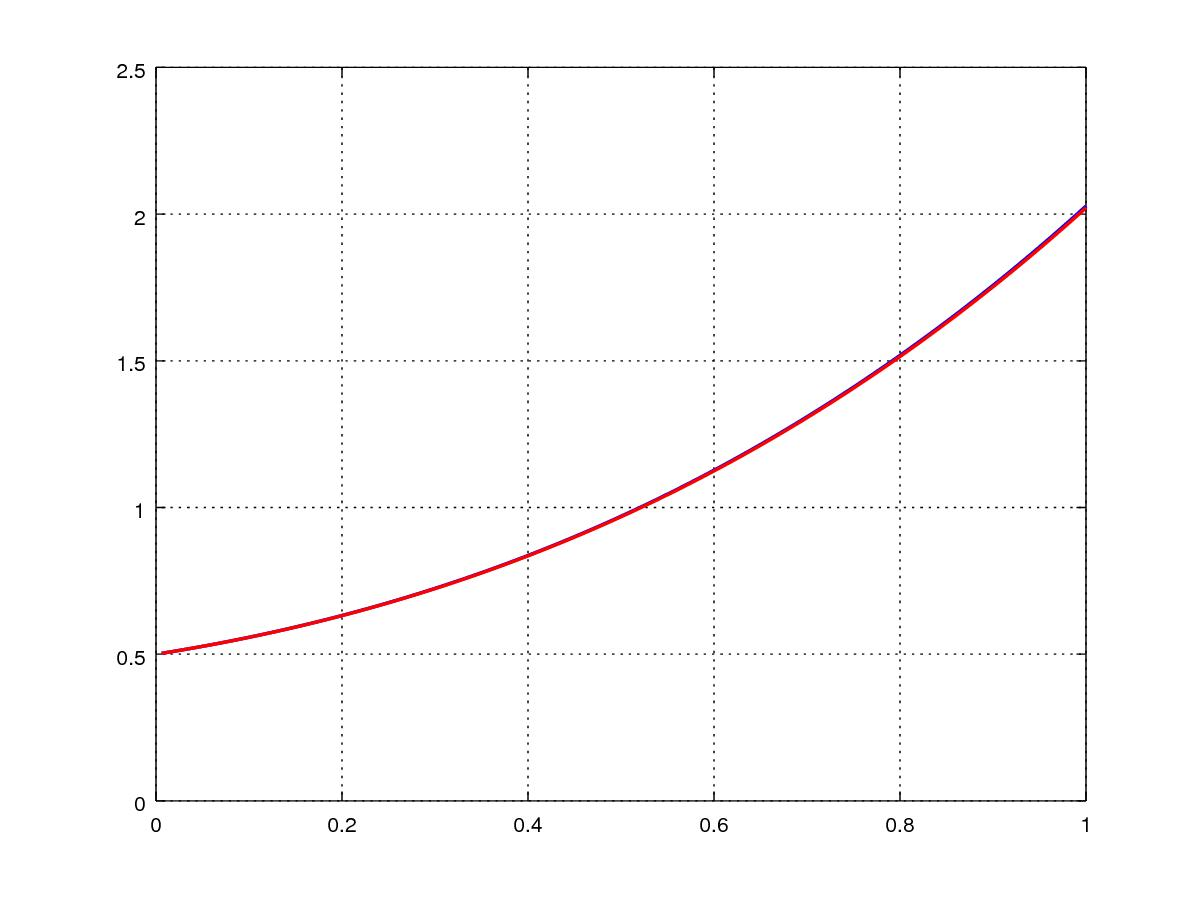
\includegraphics[width=0.8\textwidth]{./cap_pvi/dados/ex_Euler_adap/ex_Euler_adap}
    \caption{Resultados referentes ao Exemplo~\ref{ex:Euler_adap}.}
    \label{fig:ex_Euler_adap}
  \end{figure}

% \ifisoctave
% O algoritmo utilizado neste exemplo pode ser implementado no \verb+GNU Octave+ com o seguinte código:
% \begin{verbatim}
% f = @(t,y) y+sin(t);

% TOL=1e-4;
% h=1e-1;
% tf=1;

% t0=0;
% y0=0.5;

% t=[];
% y=[];

% c=1;
% do

%   h = min(h,tf-t0);
 
%   do
%     #passo h
%     y1=y0+h*f(t0,y0);
%     #passo h/2
%     y2=y0+h/2*f(t0,y0);
%     y2=y2+h/2*f(t0+h/2,y2);
%     #verifica TOL
%     est = 2*abs(y1-y2);
%     if (est > TOL)
%       h/=2;
%       if (h<1e-8)
%         error("h muito pequeno")
%       endif
%     else
%       t0+=h;
%       y0=y2;
      
%       t(c)=t0;
%       y(c)=y0;
%       c+=1;
%     endif
%   until ((est <= TOL))
  
% until (abs(t0-tf)<1e-14)

% ya = @(t) exp(t)-sin(t)/2-cos(t)/2;
% printf("%1.1E %1.5E %1.1E\n",t0,y0,abs(y0-ya(1)))

% plot(t,ya(t),'b-',t,y,'r-');grid
% \end{verbatim}
% \fi

\end{ex}

\subsection{Exercícios}

\begin{flushleft}
  [[tag:revisar]]
\end{flushleft}

\begin{exer}
  Considere o seguinte problema de valor inicial
  \begin{align}
    y' &+ e^{-y^2+1} = 2,\quad t>1,\\
    y(1) &= -1.
  \end{align}
Use o Método de Euler com passo adaptativo para computar o valor aproximado de $y(2)$. Para tanto, utilize o passo inicial $h=0,1$ e a tolerância de $TOL=10^{-4}$.
\end{exer}
\begin{resp}
  % \ifisoctave 
  % \href{https://github.com/phkonzen/notas/blob/master/src/MatematicaNumerica/cap_pvi/dados/exer_Euler_adap/exer_Euler_adap.m}{Código.} 
  % \fi
  $-5.99240\E-1$
\end{resp}
